% Szkielet dla pracy inżynierskiej pisanej w języku polskim.

\documentclass[polish,bachelor,a4paper,oneside]{ppfcmthesis}


\usepackage[utf8]{inputenc}
\usepackage[T1]{fontenc}
\usepackage{textcomp}
\usepackage{listings}
\usepackage{subfig}
\usepackage{float}
% Authors of the thesis here. Separate them with \and
\author{%
Mateusz Bartos \album{122437} \and
Piotr Falkiewicz \album{122563} \and
Aleksandra Główczewska \album{122494} \and
Paweł Szudrowicz \album{122445}}
\title{System kontroli bezpieczeństwa – The Guard}                   % Note how we protect the final title phrase from breaking
\ppsupervisor{dr inż. Mariusz Nowak} % Your supervisor comes here.
\ppyear{2018}                                         % Year of final submission (not graduation!)

\begin{document}
    % Front matter starts here
    \frontmatter\pagestyle{empty}%
    \maketitle\cleardoublepage%
    % Blank info page for "karta dyplomowa"
    \thispagestyle{empty}\vspace*{\fill}%
    \begin{center}
        Tutaj przychodzi karta pracy dyplomowej;\\oryginał wstawiamy do wersji dla archiwum PP, w pozostałych kopiach wstawiamy ksero. 
    \end{center}%
    \vfill\cleardoublepage%

    % Table of contents.
    \pagenumbering{Roman}\pagestyle{ppfcmthesis}%
    \tableofcontents* \cleardoublepage%

    % Main content of your thesis starts here.
    \mainmatter%
    \chapter{Wstęp}
Inspiracją niniejszego projektu była chęć ulepszenia istniejących systemów monitoringu o nowoczesne mechanizmy powszechnie używane w projektach programistycznych.
Nowoczesne systemy kontroli bezpieczeństwa powinny nie tylko nagrywać obraz ale także analizować go w czasie rzeczywistym i odpowiednio reagować. Na podstawie danych z kamer i czujników system powinien podejmować decyzje o stanie bezpieczeństwa domu i alarmować użytkownika o wykrytych zagrożeniach.

System kontroli bezpieczeństwa - The Guard jest naszą odpowiedzią na przedstawione problemy. Naszym celem było stworzenie systemu umożliwiającego analizę danych z czujników pomiarowych, monitorowanie pomieszczeń, w których zamontowano nasz system a także nagrywanie materiału video w momencie wykrycia ruchu i przechowywaniu go bezpiecznie na zewnętrznym serwerze aby był dostępny dla nas w każdym momencie i nie uległ zniszczeniu. Zadaniem systemu jest także poinformowanie o każdym niebezpieczeństwie właściciela systemu. Priorytetem był prosty i intuicyjny program obsługi, który mógłby być użyty przez każdą osobę, na każdej z najbardziej popularnych platform. Zdecydowano się na aplikację internetową i dwie aplikacje mobilne napisane natywnie dla systemu iOS i Android. Ponadto uzgodniono, że rozwiązanie będzie oparte na niezależnych modułach, które będzie można później, w łatwy sposób, zmodyfikować. Całość pracy jest na licencji open-source, aby każdy użytkownik mógł nie tylko korzystać z systemu ale także dowolnie go edytować.

W ramach pracy przygotowano projekt całego systemu, od urządzeń zbierających dane, przez system monitorujący i analizujący zebrane dane, po aplikacje klienckie. Następnie zaimplementowano zaprojektowane wcześniej aplikacje, złożono zestawy urządzeń składających się z Raspberry Pi 3 i czujników, oraz połączono wszystkie elementy w jeden spójny system.
Ze względu na cel pracy oraz wykorzystane technologie i usługi, zespół oparł swoją pracę o: dokumentację usług dostępną na stronach internetowych producentów, dokumentację narzędzi dołączoną do odpowiednich repozytoriów, dokumentację sprzętu.

\paragraph{Podział pracy}
\begin{itemize}
\item Mateusz Bartos: \\
Zaprojektował architekturę systemu, stworzył aplikację mobilną przeznaczoną na system Android. Ponadto przygotował maszynę wirtualną w ramach usług oferowanych przez chmurę Microsoft Azure.
\item Piotr Falkiewicz: \\
Wykonał projekt serwera obsługującego aplikacje mobilne w oparciu o protokół HTTP oraz był odpowiedzialny za przetwarzanie monitoringu dostarczanego w czasie rzeczywistym z urządzeń do aplikacji przy wykorzystaniu modułu Nginx RTMP.
\item Aleksandra Główczewska: \\
Zaprojektowała i wykonała aplikację internetową z wykorzystaniem języka Python i biblioteki Django. Odpowiedzialna za wprowadzenie uwierzytelniania użytkowników.
\item Paweł Szudrowicz: \\
Przygotował urządzenia oparte na Raspberry Pi 3 do obsługi czujników i wykonał oprogramowanie pracujące na każdym z nich. Zaprojektował i wykonał aplikację mobilną przeznaczoną na urządzenia iOS a także zaimplementował obsługę push notyfikacji wykorzystując do tego usługi Firebase.
\end{itemize}

\paragraph{Struktura pracy}
W pierwszym rozdziale opisano architekturę przygotowanego systemu. Następna część poświęcona jest opisowi kosztów utrzymania działającego systemu i wszystkich wymaganych podzespołów do jego poprawnej pracy. Kolejny dział zawiera specyfikację wykorzystanych czujników i schemat poprawnego ich podłączenia a także informacje dot. przetwarzania obrazu. W części tej poruszono również kwestię poprawnej instalacji oprogramowania na urządzeniu Raspberry Pi 3.  W czwartej części zaprezentowano użyte rozwiązania chmurowe takie jak Microsoft Azure, Firebase i omówiono działanie naszego serwera opartego na Django. Aplikacje klienckie są kolejnym tematem tej pracy. Do ich opisania wykorzystano zdjęcia ekranów z działających aplikacji i wytłumaczono najważniejsze aspekty w ich realizacji. W ostatnim dziale opisano przeprowadzone testy funkcjonalne.

    \chapter{Architektura systemu}

Wstęp do rozdziału

\section{Schemat}

// Piotr - schemat na podstawie "Praca inżynierska na Google Docs"
//tzn?

\section{Komunikacja}

Komunikacja, pomiędzy elementami systemu, odbywa się na zasadach architektury REST. Takie podejście gwarantuje prostotę przesyłanych komunikatów oraz skalowalność w kontekście nowych urządzeń Raspberry, strumieniujących dane, oraz nowych urządzeń korzystających z aplikacji klienckich. Początkowo, projekt był oparty o zapytania GET i POST.  

\paragraph{Zapytanie GET}
Metoda GET pozwala na pobranie dokumentu sieciowego, na postawie zapytania zawartego w adresie URL. Metoda ta jest używana tylko i wyłącznie do pobierania danych z punktu docelowego. 

\paragraph{Zapytanie POST}
W metodzie POST, należy zamieścić wiadomość wewnątrz zapytania HTTP. Odpowiedzią na ten typ zapytania, może być zarówno kod statusu, jak i dane, zwracane w podobnej postaci jak przy zapytaniu GET.

Wprowadzenie tokenów uwierzytelniających (więcej w akapicie nt. Bezpieczeństwa), spowodowało, że wymianę komunikatów oparto tylko i wyłącznie na zapytaniach POST. 
W zależności od zadania, obsługa zapytania polega na wykonaniu zapytania na bazie danych lub wysłaniu notyfikacji do klienta.
Obsługę zapytań można również podzielić, ze względu na zaplanowane źródło zapytania: aplikacja użytkownika lub urządzenie Raspberry.
W pierwszej kolejności przedstawione zostaną wiadomości wymieniane na linii Raspberry - Serwer.
\paragraph{a) Rejestracja Raspberry Pi:}
\begin{verbatim}
Adres: /backend/v1/devices/add
Zawartość:
{
	'serial': <serial-urządzenia>, 
	'name': <nazwa-urządzenia>, 
	'token': 'jwt.token.from.client'
}
\end{verbatim}
Działanie: Raspberry, o podanych serialu i nazwie, zostaje dodane do bazy danych urządzeń.

\paragraph{b) Wykrycie ruchu:}
\begin{verbatim}
Adres: /backend/v1/PIRnotification
Zawartość: 
{
	'serial': <serial-urządzenia>, 
	'message': <wiadomość>, 
	'token': 'jwt.token.from.client'
}
\end{verbatim}
Działanie: Po odebraniu informacji, o wykryciu ruchu, następuje pobranie klatki ze strumienia obrazu, nadawanego przez Raspberry o wskazanym serialu. Jeśli wykryto ruch człowieka, następuje nagranie fragmentu wideo, który zostaje zapisany w bazie danych Firebase Storage, a użytkownik zostaje poinformowany o zajściu i o nagraniu, któe może pobrać. Jeśli nie wykryto obecności ludzkiej, notyfikacja zostaje zignorowana.

\paragraph{c) Wykrycie zmian na czujniku:}
\begin{verbatim}
Adres: /backend/v1/notification
Zawartość: 
{
	'serial': <serial-urządzenia>, 
	'sensorType': <typ-czujnika>, 
	'value': <wartość>, 
	'token': `jwt.token.from.client`
}
\end{verbatim}
Działanie: Informuje serwer o zmianie wartości jednego z czujników.\newline
Następne zapytania dotyczą poleceń wysyłanych z aplikacji użytkownika.
\paragraph{d) Pobranie urządzeń użytkownika:}
\begin{verbatim}
Adres: /backend/v1/get
Zawartość: 
{
	'owner':<użytkownik>, 
	'token': 'jwt.token.from.client'
}
\end{verbatim}
Działanie: Zwraca listę urządzeń użytkownika.
\paragraph{e) Zmiana nazwy urządzenia:}
\begin{verbatim}
Adres: /backend/v1/devices/changeRaspName
Zawartość:
{
	'serial': <serial-urządzenia>, 
	'name': <nowa-nazwa>, 
	'token': 'jwt.token.from.client'
}
\end{verbatim}
Działanie: Zmienia nazwę urządzenia, wyświetlaną w podglądzie, w aplikacji użytkownika.
\paragraph{f) Uzbrojenie/rozbrojenie urządzenia:}
\begin{verbatim}
Adres: /backend/v1/devices/changeIsArmed
Zawartość: 
{
	'serial': <serial-urządzenia>, 
	'armed': <nowy-stan>, 
	'token': 'jwt.token.from.client'
}
\end{verbatim}
Działanie: Ustala, czy nowe powiadomienia, związane z urządzeniem, dalej będą wysyłane do aplikacji.
\paragraph{g) Pobranie listy notyfikacji:}
\begin{verbatim}
Adres: /backend/v1/devices/getNotifications
Zawartość: 
{
	'serial': <serial-urządzenia>,  
	'token': 'jwt.token.from.client'
}
\end{verbatim}
Działanie: Pobiera listę notyfikacji, powiązanych z urządzeniem o podanym serialu.
\paragraph{h) Powiązanie aplikacji z kontem użytkownika:}
\begin{verbatim}
Adres: /backend/v1/devices/fcmTokenUpdate
Zawartość: 
{
	'email': <użytkownik>, 
	'fcmToken': <token-z-firebase>, 
	'deviceId' : <id_aplikacji>
}
\end{verbatim}
Działanie: Powiązuje aplikację, zarówno mobilną, jak i sesję aplikacji przeglądarkowej, o podanym tokenie, z kontem użytkownika. Dzięki temu, notyfikacje trafiają na wszystkie urządzenia użytkownika.
\newline
\newline
Wybrane rozwiązanie pozwala na łatwą lokalizację ewentualnego błędu w działaniu systemu, oraz szybką naprawę zaistniałego problemu. Ponadto prosta logika oraz łatwe, krótkie funkcje, obsługujące zapytania, sprawiają, że dalszy rozwój tej części systemu, będzie możliwy bardzo niskim nakładem sił. 

\section{Bezpieczeństwo}

Aplikacje wysyłając zapytania do serwera, muszą potwierdzić swoją tożsamość, co dzieje się inaczej w przypadku aplikacji mobilnych i aplikacji webowej.

W~przypadku aplikacji mobilnych zastosowano proponowane przez Firebase rozwiązanie JSON Web Tokens. W~momencie wysłania zapytania POST do serwera, aplikacja wysyła także unikalny token, który następnie jest przez serwer weryfikowany przy użyciu Firebase Admin SDK.

W~przypadku aplikacji internetowej, zastosowano wbudowane w bibliotekę Django zabezpieczenia: CSRF token oraz przesyłanie id sesji wraz z zapytaniem. Zabezpieczenie CSRF tokenem uniemożliwia tzw. `Cross Site Request Forgery' tj. ataki w~których na stronie, gdzie zalogowany jest użytkownik bez jego wiedzy uruchamiany jest skrypt, najczęściej w języku JavaScript. Następnie, korzystając z~faktu, że użytkownik jest zalogowany, wysyłane jest zapytanie na serwer, które może zrobić wszystkie operacje do których upoważniony jest dany użytkownik. CSRF token zapisywany jest w przeglądarce jako `ciasteczko' (eng. cookie) i jest dołączany do danych przesyłanych w momenie kliknięcia przycisku odpowiedzialnego za przesłanie formularza. Następnie wbudowana w serwer Django biblioteka weryfikuje na podstawie zapisanych i przesłanych danych sesji poprawność tokenu i w przypadku błędu zwraca błąd serwera 403.
Ponieważ token przy każdym zapytaniu jest tworzony na nowo na podstawie otwartej sesji, rozwiązanie nie było komfortowe dla użytkowników aplikacji mobilnych: aplikacja musiałaby najpierw ustanowić połączenie z serwerem (wysłać zapytanie GET na stronę główną), następnie zalogować się (wysłać zapytanie POST z danymi logowania) oraz zapisywać tokeny i id sesji odsyłane przez serwer. Aby ograniczyć ilość zapytań wysyłanych do serwera, posłużono się powyżej opisaną metodą tokenów JWT.

    \chapter{Użytkownie}

Wstęp do rozdziału

\section{Kosztorys}
W tym podrozdziale postarano się o umieszczenie wszystkich kosztów budowy systemu i kosztów jego utrzymania. Koszt budowy systemu zależy od ilości posiadanych urządzeń pomiarowych. Zaprezentowany zostanie koszt tylko jednego urządzenia, który wygląda następująco:
\begin{enumerate}
\item Koszty czujników:
Do budowy użyto czujników: MQ-9 \cite{specyfikacjaMQ-9}, MQ-2 \cite{specyfikacjaMQ-2}, czujnik DS18B20+ \cite{specyfikacjaTemp}, czujnik ruchu \cite{pir}, czujnik wykrycia płomieni \cite {specyfikacjaFlame}. Na stronach odnośników znajdują się ich ceny ze sklepu Botland.pl. Sumaryczny koszt: 91,60 zł.
\item Koszt kamery:
Użyto kamery 5MP Full HD ze wsparciem do modułu Raspberry Pi 3. Jej koszt wynosi: 89,00zł.
\item Koszt przetwornika AC:
Użyto przetwornika MCP3008 \cite{specyfikacjaAC}. Jego koszt wynosi: 9,90zł.
\item Koszt Raspberry Pi 3 + karta pamięci 16GB: 
Ze względu na bardzo dużą ilość dostępnych źródeł jego nabycia ceny różnią się znacząco. Przyjęto ceny ze sklepu Botland.pl. Koszt: 209,90zł
\end{enumerate}
Całkowity koszt budowy jednego urządzenia wynosi zatem około 400,40zł. Oczywiście istnieje możliwość obniżenia tej ceny poprzez zakup kamery nagrywającej w mniejszej rozdzielczości.


    \chapter{Zbieranie i przetwarzanie danych z~czujników}
\section{Raspberry Pi}
Wszystkie zestawy zbudowano w~oparciu o~Raspberry Pi 3 v1.2. Zdecydowano się na to rozwiązanie, ponieważ bazuje na dystrybucji Linuxa, posiada opowiednie interfejsy i~złącza, a~także zintegrowany moduł WiFi. Minusem w~stosunku do konkurencyjnego Arduino jest brak wejść analogowych. Problem rozwiązano dodając zewnętrzny przetwornik A/C. Całość zamknięto w~małą plastikową obudowę z~wyciętymi otworami na czujniki (rys. \ref{the_guard_set}). Schemat budowy układu wykonano w~programie Fritzing (rys. \ref{the_guard_schem}).
\begin{figure}[H]
	\centering
	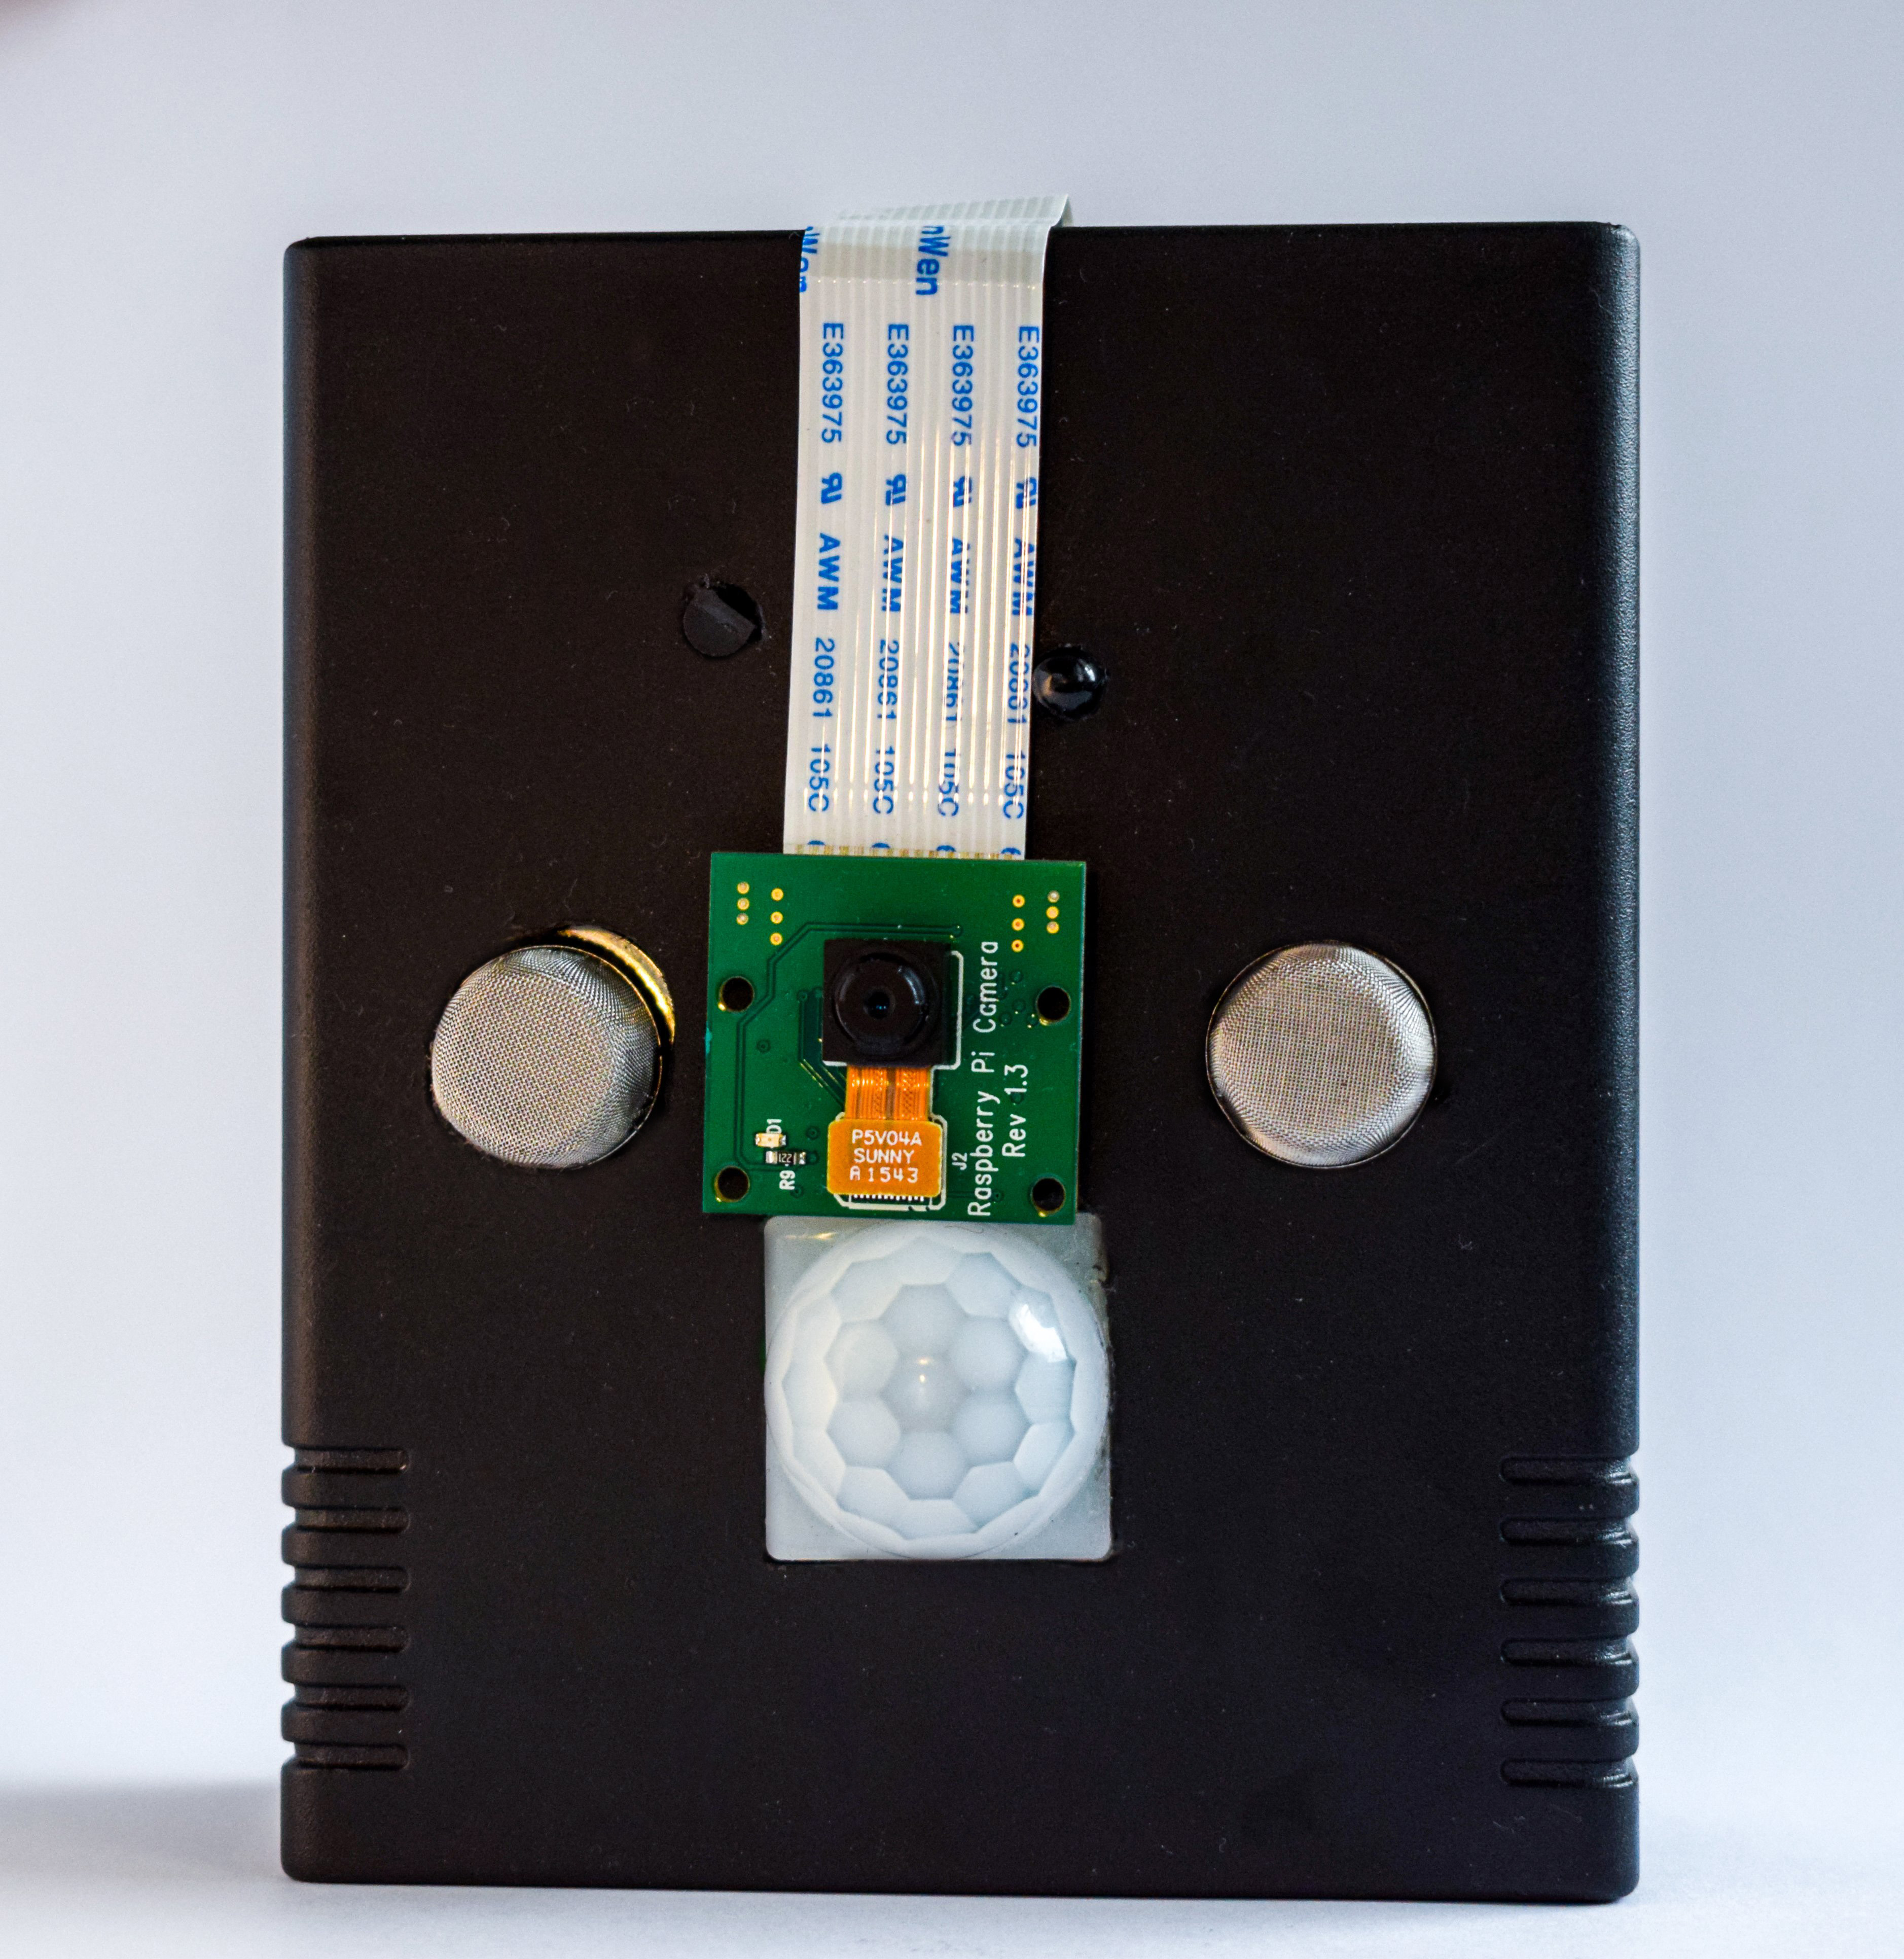
\includegraphics[width=7cm]{guard.jpg}
	\caption{Zbudowany zestaw The Guard [opracowanie własne]}
	\label{the_guard_set}
\end{figure}
\begin{figure}[H]
	\centering
	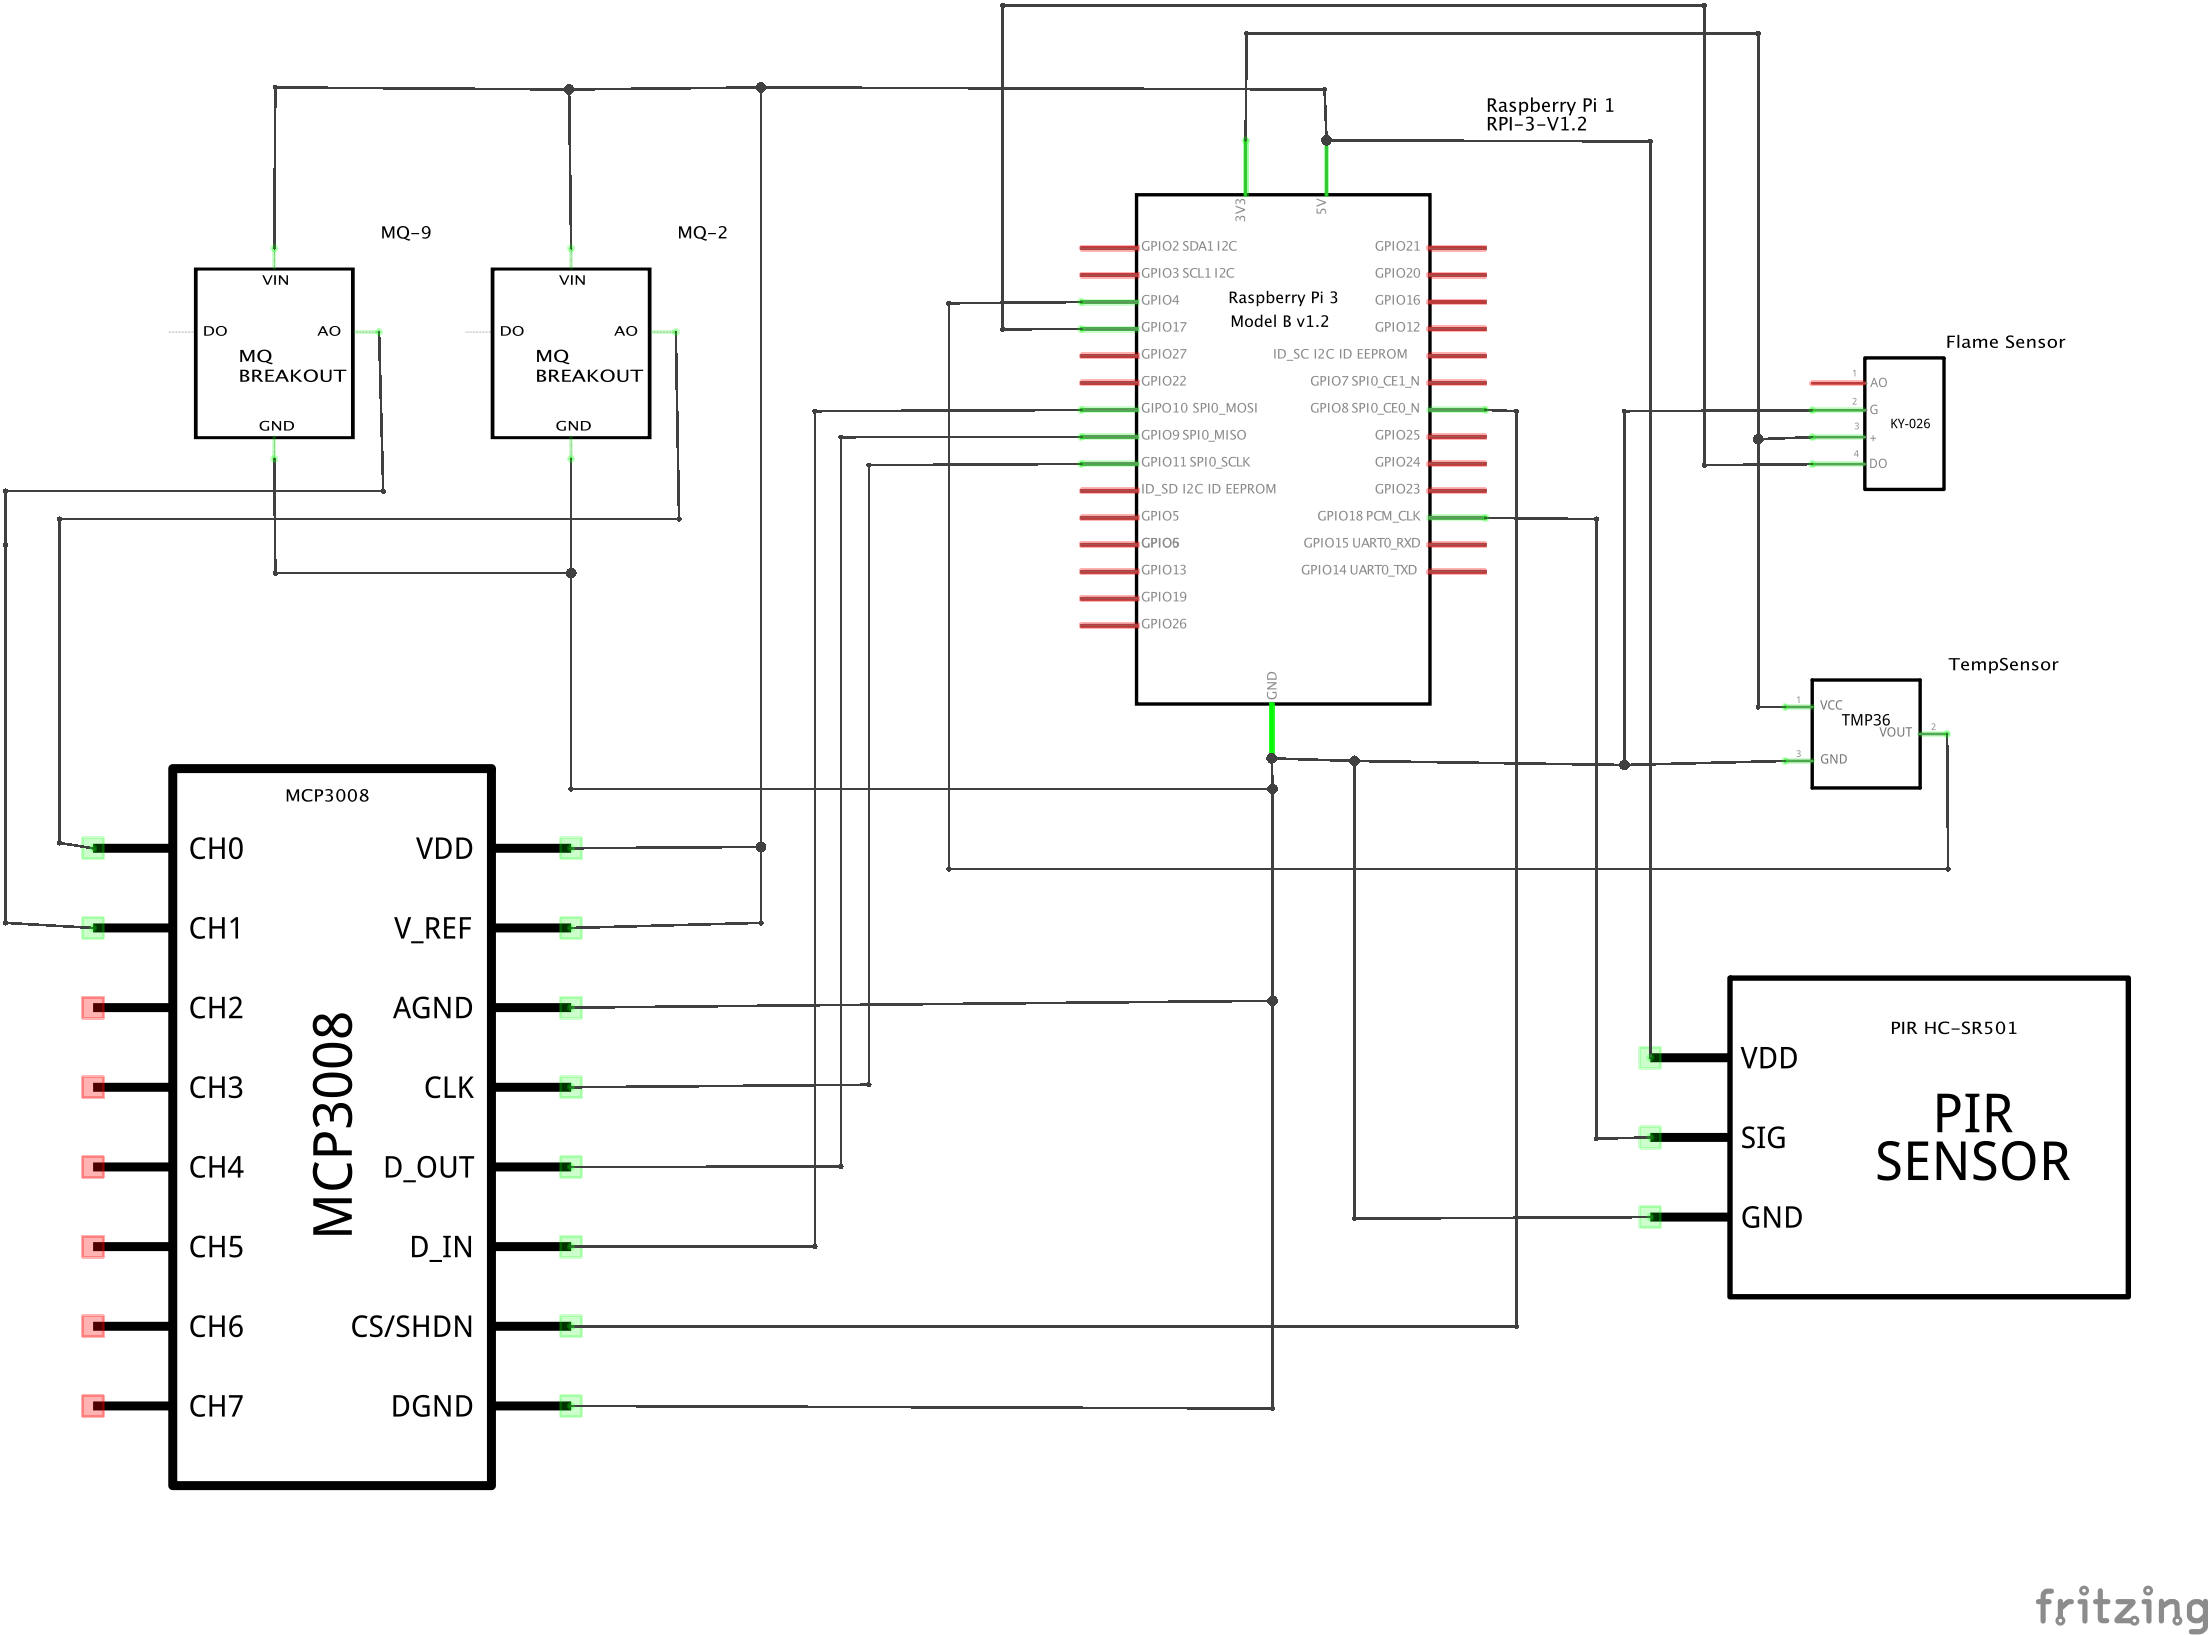
\includegraphics[width=15cm]{GuardSchem}
	\caption{Schemat układu The Guard [opracowanie własne]}
	\label{the_guard_schem}
\end{figure}
\paragraph{Specyfikacja Raspberry Pi 3 na podstawie strony Botland.com.pl \cite{specyfikacja_rasp}.}
\begin{itemize} 
\item Procesor 1.2 GHz
\item Liczba rdzeni 4. Quad Core
\item Pamięć RAM 1 GB
\item Karta pamięci microSD (w~użytych w~tej pracy urządzeniach posłużono się kartami o wielkości 8 i~16 GB).
\item 40 GPIO
\end{itemize}
Aby przygotować dowolne urządzenie Raspberry~Pi~3 do poprawnej instalacji oprogramowania The Guard należy wykonać poniższe czynności w~terminalu.
\begin{enumerate} 
\item sudo apt-get install libx264-dev
\item cd /usr/src
\item git clone git://source.ffmpeg.org/ffmpeg.git
\item sudo ./configure --arch=armel --target-os=linux --enable-gpl --enable-libx264 --enable-nonfree
\item sudo make
\item sudo install
\item sudo nano /boot/config.txt
\item w pliku config.txt dopisać Dtoverlay=w1-gpio i Gpiopin=4
\item pip intall wiringpi
\item sudo pip install spidev
\item pip install pyrebase
\end{enumerate}
Następnym krokiem jest włączenie odpowiednich interfejsów w~panelu konfiguracyjnym. Należy zmienić ustawienia zgodnie ze schematem (rys. \ref{rs_settings}).
\begin{figure}[H]
	\centering
	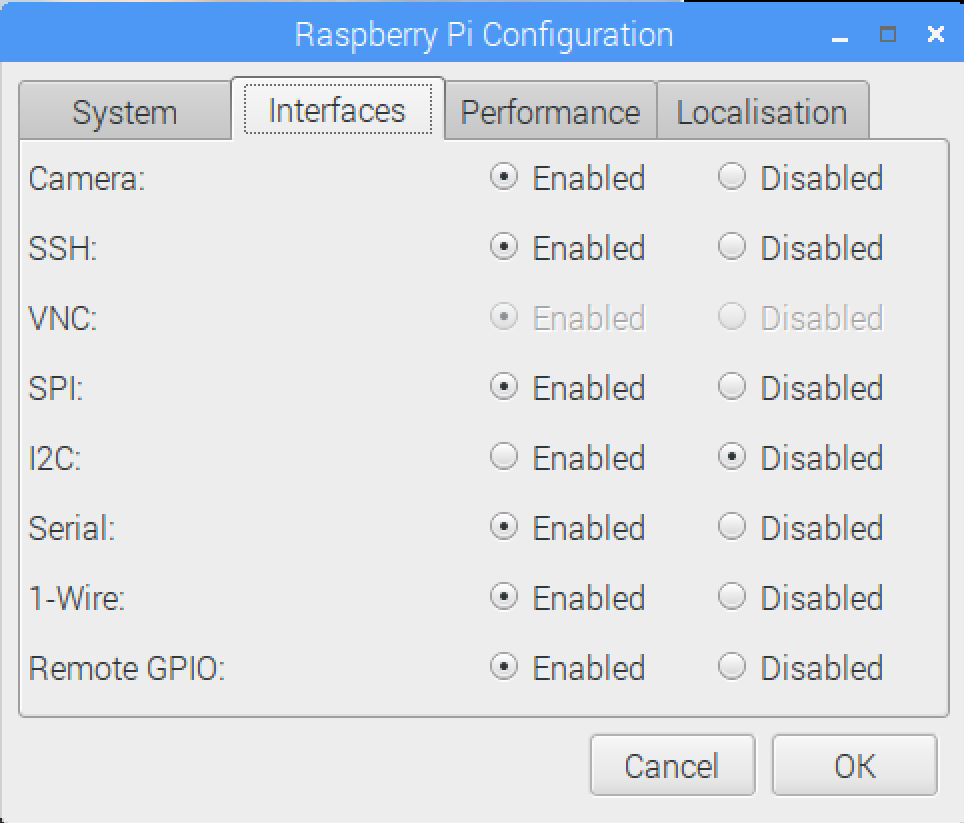
\includegraphics[width=6cm]{RSettings}
	\caption{Ustawienia [opracowanie własne]}
	\label{rs_settings}
\end{figure}
Do odczytu danych z~układów cyfrowych użyto biblioteki wiringPi. Należy podkreślić, że numeracja fizycznych pinów(rys. \ref{gpio}) i~numeracja pinów w wiringPi(rys. \ref{wiringpi}) jest różna oraz biblioteka wiringPi nie obsługuje wszystkich pinów urządzenia. Przykładowo odczyt pinu numer~1~w~wiringPi jest równoznaczny z~odczytem stanu pinu numer 12 (GPIO18).
\begin{figure}[H]
    \centering
    \subfloat[GPIO]{
	    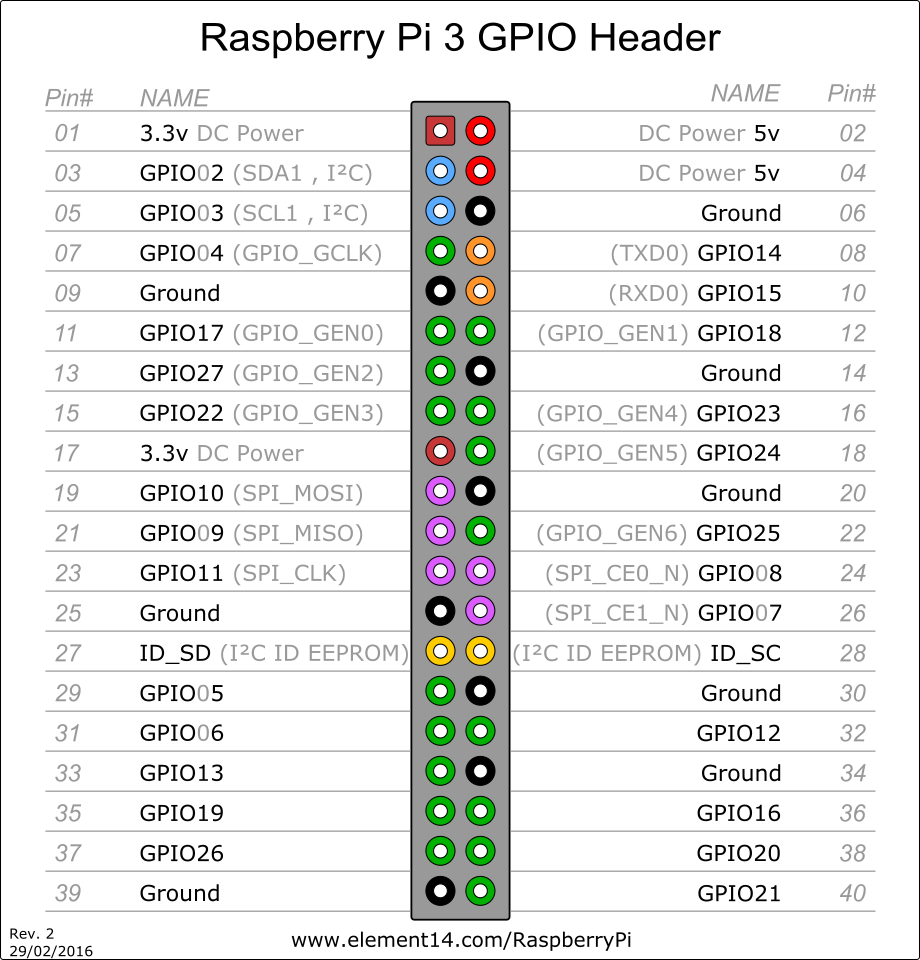
\includegraphics[width=5cm]{gpio.png}
	    \label{gpio}
	}
    \hspace{3cm} 
    \subfloat[WiringPi]{
	    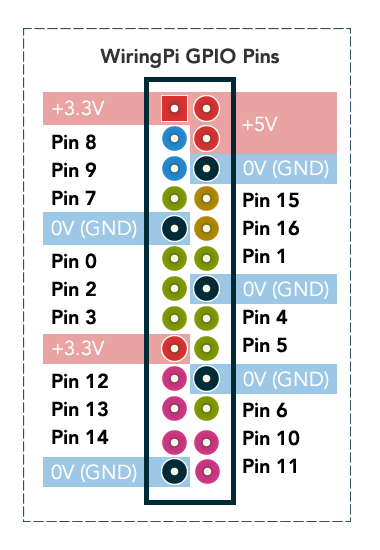
\includegraphics[height=5cm]{wiringpi.png}
	    \label{wiringpi}
	    }
    \caption{Porównanie pinów Raspberry Pi 3 \cite{gpio} z pinami wiringPi \cite{wiringpi}}
    \label{piny}
\end{figure}

Zainstalowane oprogramowanie odpowiedzialne jest za ciągłe monitorowanie stanów i~zbieranie danych z~czujników pomiarowych. Po podłączeniu układu do zasilania program jest uruchamiany automatycznie. Pierwszą czynnością jaką wykonuje Raspberry Pi jest wysłanie swojego numeru seryjnego do bazy danych Firebase. Cały proces jest w~pełni zautomatyzowany. Dzięki temu użytkownicy od razu mogą dodać urządzenie i~przeglądać dane z~czujników na aplikacjach klienckich. Dodanie akcesorium pomiarowego następuje poprzez wprowadzenie w~aplikacji jego numeru seryjnego.
\section{Czujniki}
Każdy zestaw składa się z~5~czujników, jednej kamery oraz jednego przetwornika analogowo-cyfrowego (AC). 
\paragraph{a) Specyfikacja MQ-9 - czujnik tlenku węgla\cite{specyfikacjaMQ-9}.}
\begin{itemize} 
\item Zasilanie: 5~V
\item Pobór prądu: 150 mA
\item Temperatura pracy: od -10 do 50 \textdegree{}C
\item Wyjścia: analogowe oraz cyfrowe (do pomiarów użyto wyjścia analogowego)
\end{itemize}
\paragraph{b) Specyfikacja MQ-2 - czujnik LPG i dymu \protect\cite{specyfikacjaMQ-2}.}
\begin{itemize} 
\item Zasilanie: 5~V
\item Pobór prądu: 150 mA
\item Temperatura pracy: od -10 do 50 \textdegree{}C
\item Wyjścia: analogowe oraz cyfrowe (do pomiarów użyto wyjścia analogowego)
\end{itemize}
\paragraph{c) Specyfikacja czujnika wykrywania płomieni \protect\cite{specyfikacjaFlame}.}
\begin{itemize} 
\item Zasilanie: 3.3 V
\item Zakres wykrywanej fali: 760 do 1100nm
\item Kąt detekcji: od 0 do 60 stopni
\item Temperatura pracy: od -25 do 85 \textdegree{}C
\end{itemize}
\paragraph{d) Specyfikacja DS18B20 - czujnik temperatury \protect\cite{specyfikacjaTemp}.}
\begin{itemize} 
\item Zasilanie: 3.3 V
\item Zakres pomiarowy: od -55 do 125 \textdegree{}C
\end{itemize}
\paragraph{e) Kamera:}
\begin{itemize} 
\item Wykorzystano moduł kamery Raspberry Pi
\item Kamera 5MP - wspierająca nagrywanie 30 klatek na sekundę w rozdzielczości Full HD
\end{itemize}
\paragraph{f) Specyfikacja MCP3008 - przetwornik A/C \protect\cite{specyfikacjaAC}.}
\begin{itemize} 
\item Zasilanie: od 2.7V do 5.5V
\item Pobór prądu: 0.5 mA
\item Interfejs komunikacyjny: SPI
\item Liczba kanałów: 8
\item Rozdzielczość: 10bit
\end{itemize}
\paragraph{g) Specyfikacja czujnika ruchu PIR HC-SR501 \protect\cite{pir}.}
\begin{itemize} 
\item Zasilanie: od 4.5V do 20V
\item Pobór prądu w stanie czuwania: 50 uA
\item Zakres pomiarowy: maks. 7 m
\item Kąt widzenia: do 100\textdegree{}
\end{itemize}
Na wykresach (rys. \ref{mq2}, rys. \ref{mq9}) przedstawiono charakterystyki czułości czujników.
\begin{figure}[ht]
	\centering
	\subfloat[Charakterystyka czujnika MQ-2 \protect\cite{mq2}]{
	    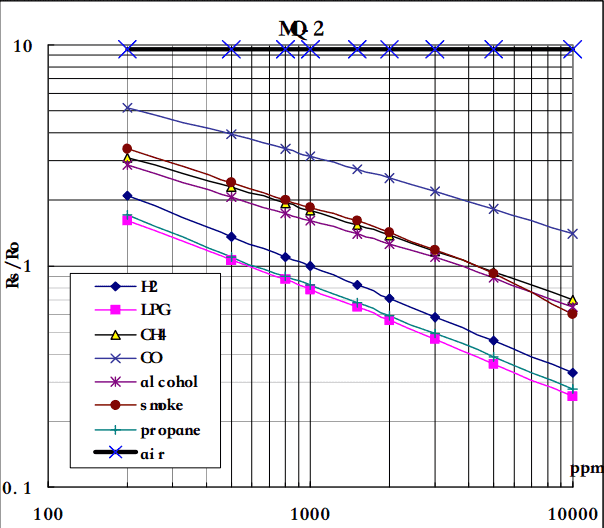
\includegraphics[height=6cm]{MQ2}
	    \label{mq2}
	}
	\hfill
	\subfloat[Charakterystyka czujnika MQ-9 \protect\cite{mq9}]{
	    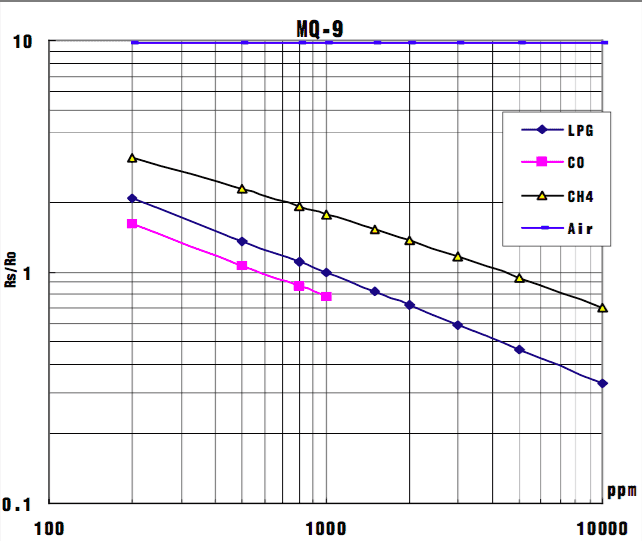
\includegraphics[height=6cm]{MQ9}
	    \label{mq9}
	    }
	\caption{Charakterystyka czujników MQ-2 oraz MQ-9.}
	\label{mq2_mq9}
\end{figure}
\\Ro - jest to stała wartość oporu czujnika przy 1000ppm H2 w~czystym powietrzu.\\
Rs - jest to opór czujnika w~różnych stężeniach gazu. \\
Przy założeniu stałej wartości Ro, przy wzroście Rs czułość czujnika maleje -~im mniejszy stosunek Rs do Ro tym dokładniejszy pomiar wykonywany przez czujnik. Na schemacie \ref{mq2_mq9} widać, że obydwa czujniki reagują na wiele różnych gazów. MQ-2 nazwano w tej pracy czujnikiem LPG, a~MQ-9 czujnikiem CO ze względu na to, że w~stosunku do tych gazów mają najwyższą czułość. 

Żaden z modeli Raspberry nie posiada wbudowanego przetwornika analogowo-cyfrowego dlatego konieczne było użycie układu zewnętrznego. Wybrano przetwornik MCP3008 ze względu na jego nisko koszt i~komunikację poprzez interfejs SPI, który jest wspierany przez Raspberry Pi. MCP3008 to 10-bitowy przetwornik analogowo-cyfrowy zasilany napięciem 5V.  Przetwornik 10-bitowy jest w~stanie rozróżnić 1024 stany. Posiada 8 kanałów jednak w~projekcie wykorzystano tylko 2~–~dla MQ-9 i~MQ-2.
\paragraph{Interfejs SPI:}
\begin{figure}[ht]
	\centering
	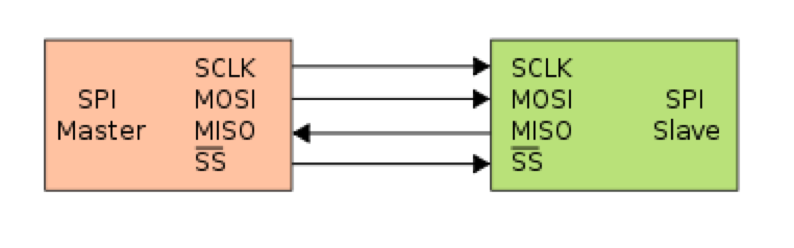
\includegraphics[width=7cm]{SPI.png}
	\caption{Interfejs SPI \protect\cite{spi}}
	\label{spi}
\end{figure}
SPI jest to interfejs synchroniczny (rys. \ref{spi}). Może być do niego podłączone wiele urządzeń typu Slave, jednak są połączone tylko z~jednym urządzeniem Master, które generuje sygnał zegarowy. Urządzenie typu Master poprzez linię SS wybiera urządzenie z~którym chce się komunikować. \\
Interfejs SPI zawiera jeszcze 3~linie.
\begin{enumerate} 
\item MOSI (ang. Master Output Slave Input). \\
Poprzez tę linię wysyłane są dane z~Raspberry Pi do przetwornika analogowo cyfrowego MCP3008.
\item MISO (ang. Master Input Slave Output).\\
Poprzez tę linię wysyłane są dane z~przetwornika AC do układu Master, czyli w~naszym przypadku Raspberry~Pi~3.
\item SCLK (ang. Serial Clock).\\
Ta linia wykorzystywana jest do przesłania zegara wygenerowanego przez Rapberry~Pi~3.
\end{enumerate}
Do komunikacji poprzez ten interfejs wykorzystano bibliotekę SpiDev \cite{spidev}. \\
Każdy układ monitoruje wskaźniki pomiarowe z czujników analogowych i~cyfrowych. W~przypadku wykrycia wskazań, które w~znaczący sposób odbiegają od normy informuje właściciela o~zagrożeniu. Informacja ta wysyłana jest do wszystkich urządzeń(smartfony, tablety itp), które posiada właściciel.  Analizując dane z~czujników analogowych w~czystym powietrzu, które wynoszą odpowiednio:\\
czujnik MQ-9: od 0.15 do 0.2,\\
czujnik MQ-2: od 0.05 do 0.15,\\
przyjęto, że granicą wysłania notyfikacji do użytkownika jest przekroczenie progu 0.3. Wartości te to znormalizowane dane z~przetwornika AC, który jak już wcześniej wspomniano wykrywa 1024 stany. Odczytywane wartości bezpośrednio na wyjściu przetwornika MCP3008 dla czujnika MQ-9 w~czystym powietrzu to około 170. Stąd 170/1024 = 0.166. Wysłanie notyfikacji wiąże się z~otrzymaniem wartości większej niż 308.

Czujniki cyfrowe wykorzystane w~pracy informują o~wykryciu płomieni lub ruchu. Czujnik ruchu wykrycie zagrożenia określa przez stan wysoki, natomiast czujnik płomieni przez stan niski. Przy implementacji zanegowano sygnał odbierany z~czujnika płomieni, aby stan wysoki zawsze informował o~niebezpieczeństwie, a~stan niski reprezentował jego brak. Na czujnikach znajduje się potencjometr, za pomocą którego dowolnie można ustawiać jego czułość. Odczyt danych następuje nieprzerwanie co 2~sekundy. Nie należy obawiać się, że aplikacja nie odczyta zagrożenia z~powodu zbyt krótkiego trwania sygnału wysokiego w bazie danych, ponieważ czujnik utrzymuje stan wysoki przez 5~sekund po wykryciu ruchu. 

Oprogramowanie wysyła także informacje z~czujników do bazy danych Firebase. Zastosowanie takiej bazy daje możliwość monitorowania wszystkich danych w~czasie rzeczywistym na aplikacjach klienckich. Dodatkowo w~przypadku zagrożenia czyli przekroczeniu progu, o~którym mowa wyżej wysyłana jest push notyfikacja do urządzeń użytkownika, a~informacja o~zagrożeniu zapisywana jest w~bazie danych Django. Każdy użytkownik jest w~stanie odtworzyć całą historię wydarzeń w~swoim systemie.

Aby zapewnić wydajny i~pewny system bezpieczeństwa przy otrzymaniu wysokich wartości na czujnikach zapisywany jest czas zdarzenia. Każda kolejna notyfikacja zostanie wysłana po upływie 10 minut od poprzedniej przy założeniu, że stan na czujniku nadal jest wysoki. 

\section{Obsługa wideo}

\paragraph{Protokół RTMP}
Podstawą funkcji strumieniowania wideo jest protokół RTMP (ang. Real-Time Message Protocol). Jest to oparty na protokole TCP protokół wysyłania obrazu, dźwięku oraz danych. \cite{MOBILERTMP}
Podstawową jednostką danych w~protokole RTMP jest wiadomość (ang. Message), której struktura jest zależna od typu strumieniowanych informacji. 
Wiadomości dzielone są na części (ang. Chunks), które są gotowe do transmisji. Strumień RTMP to ostatecznie strumień fragmentów wiadomości (ang. Chunk Stream) \cite{STREAMRTMP}.

Ponadto wykorzystano protokół HLS (HTTP Live Streaming), którego cechą jest zapisywanie odbieranego obrazu w plikach o~określonej długości. Gdy aplikacja kliencka odtwarza strumień wideo, w~rzeczywistości odbiera strumieniowane po kolei zapisane pliki .ts. Zaletą takiego rozwiązania jest płynność odbieranego wideo, a~jego wadą opóźnienie w~transmisji.

\paragraph{H264}
W~pracy wykorzystano kodowanie obrazu zgodnie ze standardem H.264. Charakteryzuje go niska złożoność algorytmów kompresji oraz niewielkie opóźnienie dzięki czemu idealnie nadaje się do zadań związanych z~szybkim enkodowaniem obrazu przed wysłaniem. \cite{H264}
Cechą charakterystyczną dla tego typu kodowania wideo jest użycie klatki kluczowej (ang keyframe, i-frame). Jest to pełna klatka obrazu, podczas gdy następujące po niej dane wyrażają różnice między dwoma tą a~następnymi klatkami. Rozwiązanie to pozwala to na zmniejszenie rozmiarów ostatecznego obrazu wideo.

\paragraph{Raspberry Pi}
Do obsługi odbioru strumienia wideo po stronie Raspberry Pi wykorzystywane jest narzędzie ffmpeg, które pozwala na przechwytywanie obrazu z kamery, ustawianie własności wysyłanego obrazu oraz punktu docelowego na który ten obraz będzie przesłany.

Pobranie numeru seryjnego urządzenia i użycie go, jako fragment adresu końcowego, gwarantuje stworzenie unikatowego dla każdego urządzenia adresu. Poniżej przedstawiono skrypt wykonujący wymienione zadania. Do pobrania obrazu z~kamery Raspberry pi posłużono się narzędziem raspivid. \cite{raspivid}
\begin{verbatim}
#!/bin/bash
serial_id="$(cat /proc/cpuinfo | grep Serial | cut -d ' ' -f 2)"
raspivid -o - -t 0 -fps 30 -b 1000000 | ffmpeg -re -ar 44100 -ac 2 
-acodec pcm_s16le -f s16le -i /dev/zero -f h264 -i - -vcodec copy -g 60 
-strict experimental 
-f flv rtmp://52.236.165.15:1936/camera/${serial_id}
\end{verbatim}
Pierwszą czynnością wykonywaną w~skrypcie jest otwarcie pliku /proc/cpuinfo. Następnie znajdowana jest w~nim linia, w~której znajduje się unikalny serial urządzenia. Następnie, z~wykorzystaniem potoku i~funkcji cut wartość ta zostaje przypisana do zmiennej serialid.

\begin{itemize}
\item Pierwszym przełącznikiem jest -o oraz parametr -. Oznacza to, że obraz z kamery jest wysyłany na wyjście standardowe.
\item Przełącznik -t ustawiony na 0~pozwala przekazywać obraz z~modułu kamery przez nieokrelony czas. Aby przestać pobierać wideo, należy użyć przerwania za pomocą sygnału SIGINT (obsługiwanego w terminalu skrótem klawiszowym CTRL+C).
\item Opcja -fps pozwala wskazać liczbę przechwytywanych klatek w~ciągu sekundy. Tutaj wykorzystano maksymalne możliwości wybranego modułu kamery.
\item Ostatnią opcją, wykorzystaną w~pobieraniu obrazu z kamery, jest bitrate, tzn wielkość jednostki pamięci w~której ma się znaleźć obraz przechwycony w~ciągu 1~sekundy strumienia. Ustawienie opcji -b~na 1000000 oznacza, że 1~sekunda wideo, może zajmować 125 kilobajtów pamięci. Jest to szczególnie istotna informacja w~kontekcie transmisji obrazu poza urządzenie przy wykorzystaniu łącza internetowego.
\end{itemize}

Drugim poleceniem jest wywołanie narzędzia ffmpeg. Odbiera ono za pomocą potoku przechwytywany obraz i~przekazuje go na docelowy punkt końcowy. Za jego pomocą ustalane są ostateczne opcje kodujące obraz w~trakcie transmisji.
\begin{itemize}
	\item Przełącznik -re pozwala odczytywać dane wejściowe z~oryginalną częstotliwością. (W powyższym skrypice zostają przechwycone ustawienia przełącznika narzędzia raspivid -fps 30).
\item Opcje  -ar, -ac, -acodec, -f, -strict odpowiadają kolejno za: próbkowanie dźwięku, wybór liczby kanałów, kodek audio, format dźwięku oraz wybór eksperymentalnego sposobu kodowania. Wymuszenie wykorzystania, jako wejścia strumienia dźwięku, na /dev/zero, oznacza, że strumień ten zostaje wypełniony wartościami pustymi. Zatem opcje transmisji dźwięku są nieistotne.
\item Przełącznik -vcodec ustala kodek wideo. W~pracy wykorzystano standard kodowania H.264.
\item Następnie ustawiono wejście obrazu. Przełącznik -i - powoduje, że narzędzie ffmpeg przechwytuje, dzięki potokowi, obraz przekazywany funkcją raspivid.
\item Opcja -g 60 oznacza, że tzw klatka kluczowa (ang. keyframe) pojawia się co 60 klatek (w~tej sytuacji co 2 sekundy). 
\item Przełącznik -f w~przypadku strumienia obrazu z~kamery wymusza format nadawanego wideo.  
\item Ostatnim elementem polecenia jest podanie punktu docelowego dla strumienia. Za pomocą protokołu RTMP, obługiwanego przez serwer o~adresie IP 52.236.165.15 na porcie 1936, obraz wysyłany jest na aplikację o~nazwie camera i~punkt charakteryzowany przez numer seryjny urządzenia. Działanie tego elementu opisano w kolejnym punkcie. 
\end{itemize}

\paragraph{Serwer}
Narzędziem umożliwiającym obsługę proxy jest serwer nginx. W~części projektu związanej ze strumieniowaniem wideo wykorzystano moduł nginx-rtmp \cite{NGINX}. Umożliwia on obsługę obrazu transmitowanego z~wielu źródeł, na wiele urządzeń równocześnie. 
Moduł ten pozwala na realizację wielu funkcji, a niektóre z nich przedstawiono poniżej.
\begin{itemize}
\item Tworzenie dynamicznych punktów końcowych, dla urządzeń strumieniujących obraz.
\item Zmianę parametrów przechwytywanego obrazu .
\item Zapisywanie nagrań po stronie serwera.
\item Tworzenie punktów nadających, dla aplikacji odtwarzających strumień.
\end{itemize}
Ponadto pozwala na utworzenie aplikacji HLS przechowującej tymczasowo obraz, zanim zostanie on przesłany dalej. Pozwala to na uniknięcie opóźnień między kolejnymi klatkami obrazu.

Wszystkie funkcjonalności są zdefiniowane poprzez ustawienia pliku konfiguracyjnego, którego lokalizacja to /usr/local/nginx/conf/nginx.conf:

\begin{verbatim}
rtmp {
    server {
            listen 1936;
            chunk_size 4096;
            application camera {
                    hls on;
                    hls_path /mnt/hls/;
                    hls_fragment 2;
                    hls_playlist_length 3;
                    allow publish all;
                    allow play all;
                    live on;
                    record off;
             }
    }
}
\end{verbatim}

Powyższy plik koniguracyjny powoduje, że serwer rtmp dostępny jest na porcie 1936 (domyślne porty dla protokołu RTMP na urządzeniach z~systemem z~rodziny Ubuntu to 1935 i~1936). Następnie tworzona jest aplikacja o~nazwie camera. Dla aplikacji wysyłających dane, jest ona dostępna pod adresem: rtmp://<ip-serwera>:1936/camera/<klucz>, gdzie klucz jest wybierany przez aplikację i~tworzony dynamicznie, gdy tylko urządzenie zacznie nadawać dane pod wskazany adres.
Ustawienia aplikacji decydują o~tym, że dla urządzeń odtwarzających wideo, dostępne jest ono dzięki aplikacji HLS - opcja hls on. Na szczególną uwagę zasługują linie: hls~fragment~2~oraz hls~playlist~length~3, które wskazują na to, że po stronie serwera nagrywane są 2~tymczasowe fragmenty, o~długości 3~sekund każdy. Pliki te są przechowywane w~folderze /mnt/hls/, a~ich nazwę jednoznacznie będzie wskazywać klucz strumienia.

\begin{verbatim}
http {
    server {
        listen       80;
        location /hls {
                types {
                        application/vnd.apple.mpegurl m3u8;
                        video/mp2t ts;
                }
        root /mnt/;
        }
    }
}
\end{verbatim}

Konfiguracja ta udostępnia aplikację HLS. Dla aplikacji klienckich, obraz będzie dostępny pod adresem: http://<ip-serwera>:80/hls/<klucz>.m3u8, o~czym decyduje konfiguracja części związanej z serwerem RTMP.


    \chapter{Rozwiązania chmurowe}

\section{Microsoft Azure}

Aby zapewnić wysoki poziom bezpieczeństwa oraz dostępności systemu zdecydowano się na skorzystanie z chmury Micrsoft Azure.

\section{Firebase}

// Mateusz

\section{Aplikacja serwerowa}

// Ola

\section{Baza danych}

// Ola

    \chapter{Aplikacje klienckie}

Na podstawie analizy statystyk dotyczących podziału rynku aplikacji na platformy, dostępnych na stronie statcounter.com \url{http://gs.statcounter.com/os-market-share/mobile-tablet/worldwide/#monthly-201801-201801-bar} , zdecydowano się na stworzenie 3 klientów systemu The Guard, które pozwolę możliwie największej grupie osób na korzystanie z systemu:
\begin{itemize}
\item aplikacja mobilna na system Android,
\item aplikacja mobilna na system iOS,
\item aplikacja webowa.
\end{itemize}

\section{Funkcje aplikacji}
\paragraph{Logowanie}
Do prawidłowego przejścia do ekranu głównego aplikacji niezbędne jest posiadanie konta. Po rejestracji użytkownika lub po pomyślnym uwierzytelnieniu jeśli konto zostało już wcześniej założone następuje pobranie wszystkich danych użytkownika, jego podłączonych urządzeń i przejście do głównego panelu z dostępem do wszystkich niżej omówionych funkcji.
\nopagebreak
\begin{figure}[H]
   \centering
   \subfloat[Aplikacja Android]{
\includegraphics[height=5cm]{android-screenshots/Logowanie.png}}
   \hfill
   \subfloat[Aplikacja iOS]{
\includegraphics[height=5cm]{ios_screenshots/login.png}}
   \hfill
   \subfloat[Aplikacja webowa]{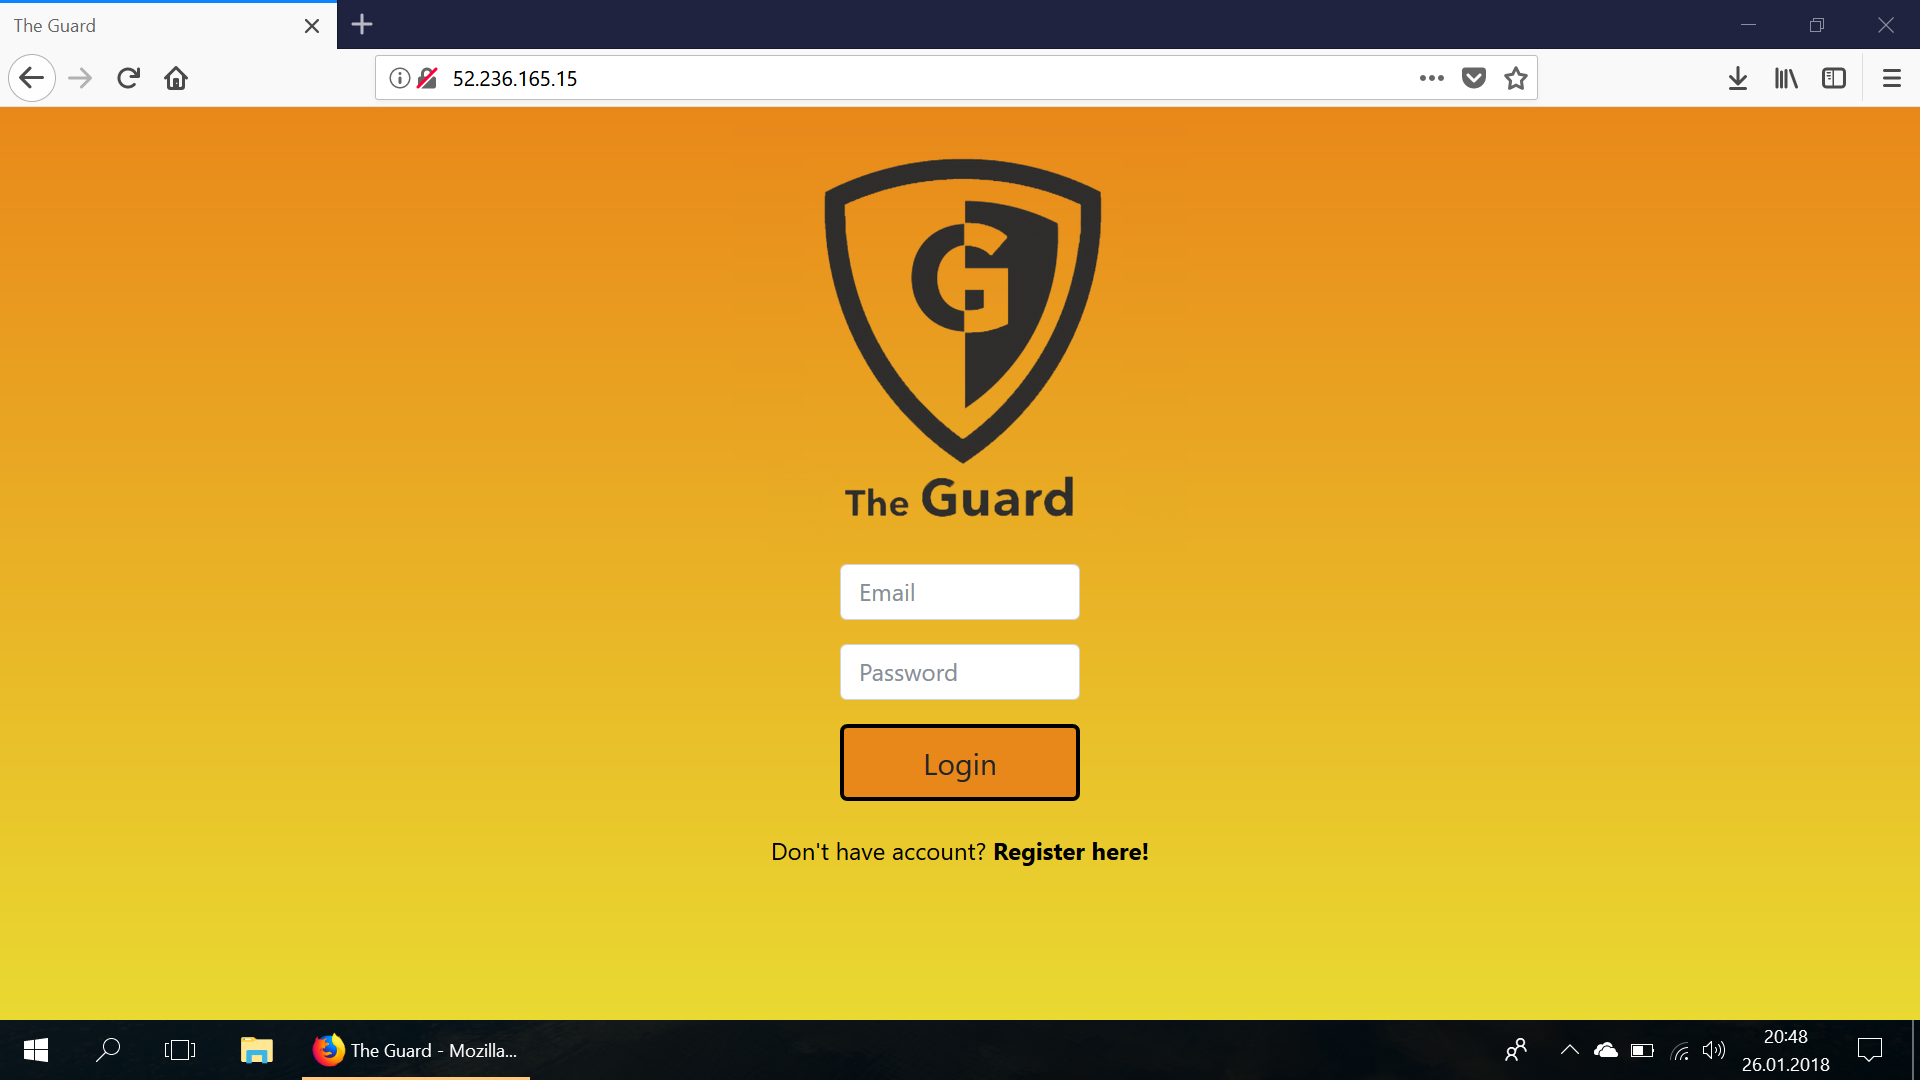
\includegraphics[height=4cm]{web_screenshots/login.png}}
   \caption{Widok logowania}
   \label{fig:logowanie}
\end{figure}

\paragraph{Monitoring}
Aplikacja pobiera i wyświetla obraz na żywo z zaznaczonego urządzenia podłączonego do konto użytkownika.
\nopagebreak
\begin{figure}[H]
    \centering
    \subfloat[Aplikacja Android]{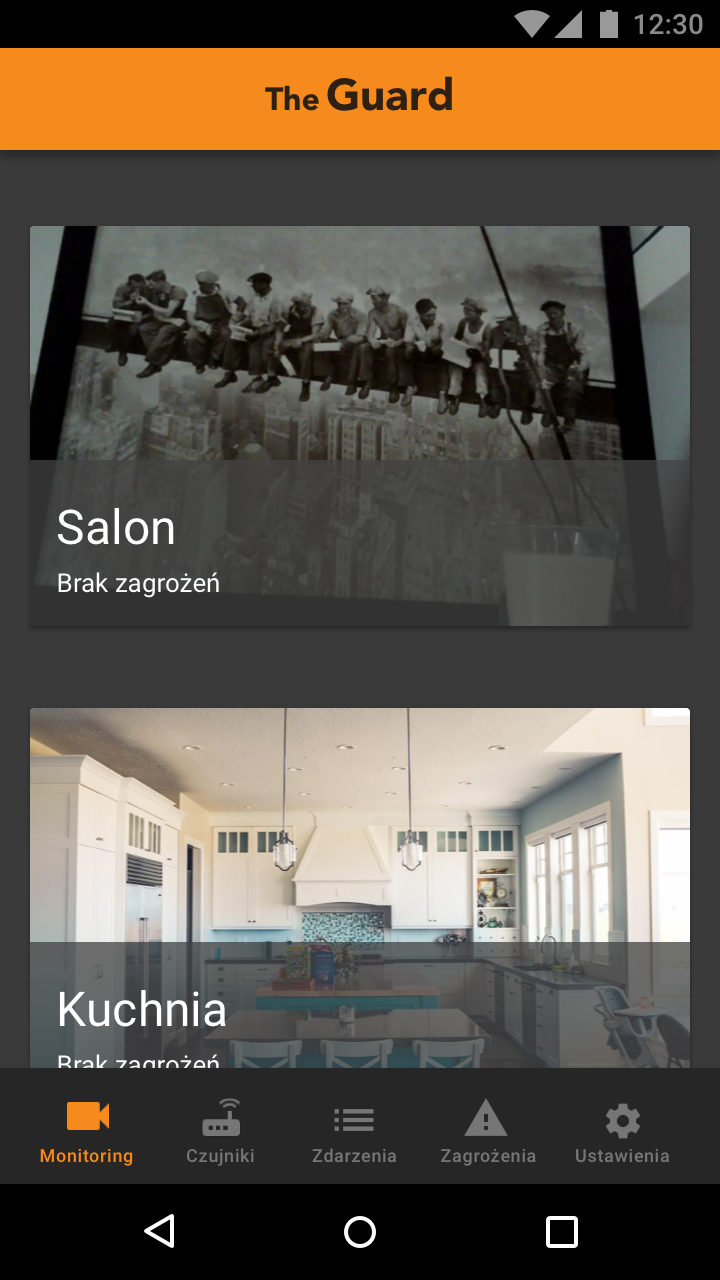
\includegraphics[height=5cm]{android-screenshots/Monitoring.png}}
    \hfill
    \subfloat[Aplikacja iOS]{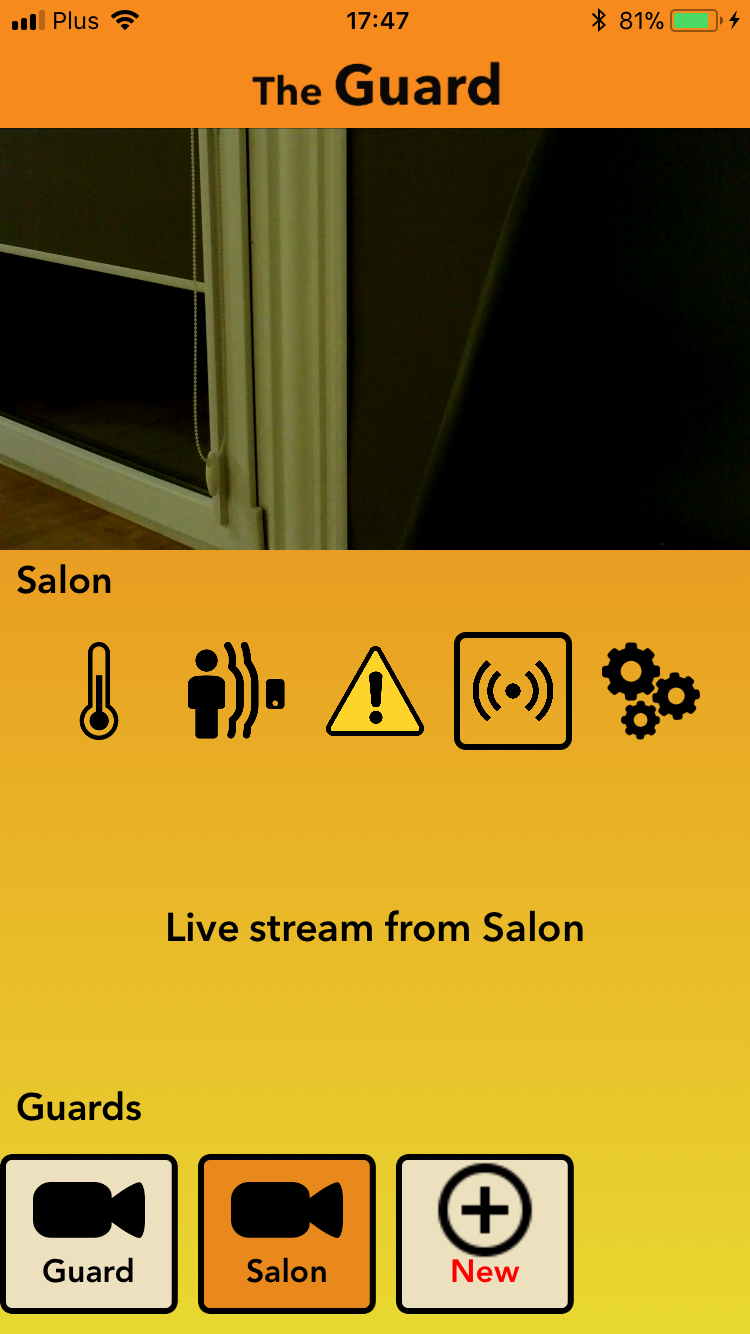
\includegraphics[height=5cm]{ios_screenshots/liveStreamiOS.png}}
    \hfill
    \subfloat[Aplikacja webowa]{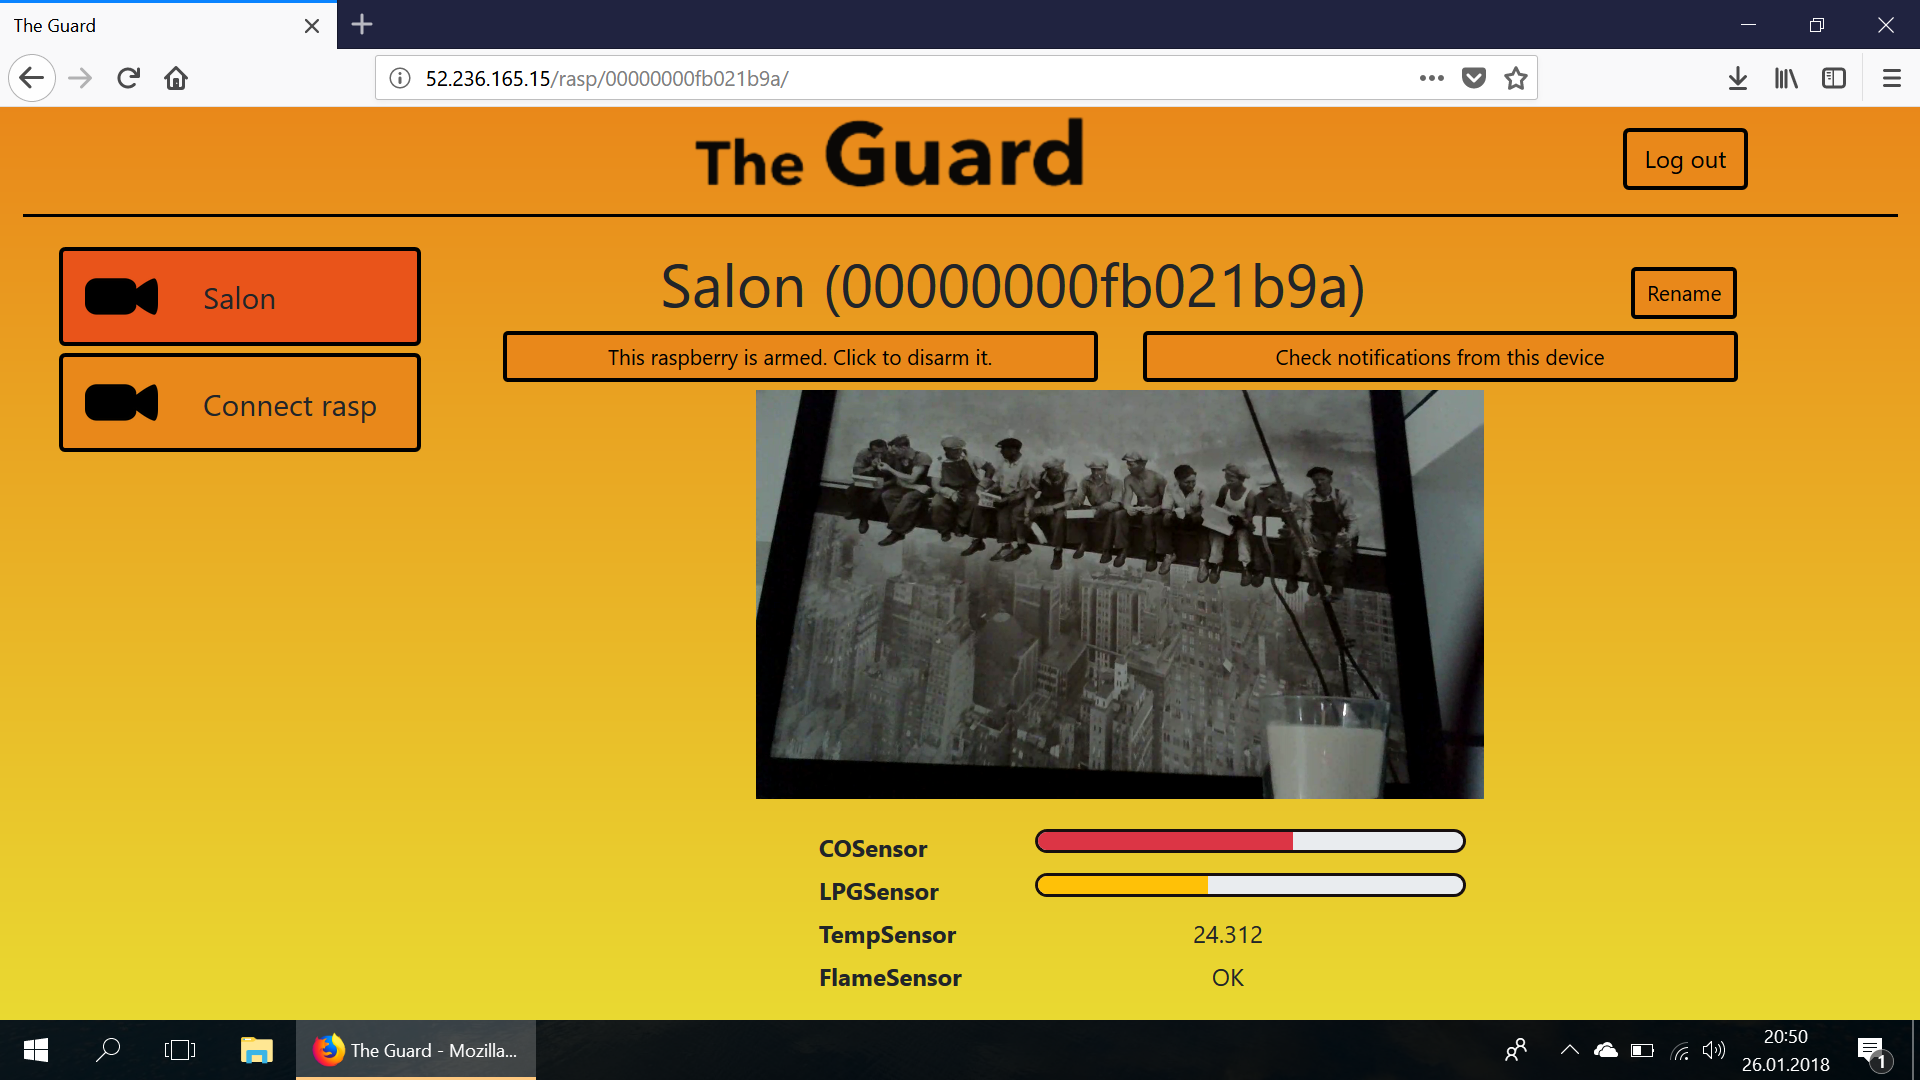
\includegraphics[height=4cm]{web_screenshots/rasp_view.png}}
    \caption{Widok monitoringu}
    \label{fig:monitoring}
\end{figure}

\paragraph{Status czujników}
Po przejściu do tej sekcji użytkownik otrzymuje bieżące dane z wszystkich czujników z zaznaczonego urządzenia. Na podstawie koloru prezentowanej wartości z czujnika użytkownik może analizować zagrożenie. Kolor zielony reprezentuje bezpieczne odczyty na czujnikach, kolor pomarańczowy średnie, kolor czerwony natomiast oznacza bardzo wysoki poziom niebezpieczeństwa.
\nopagebreak
\begin{figure}[H]
    \centering
    \subfloat[Aplikacja Android]{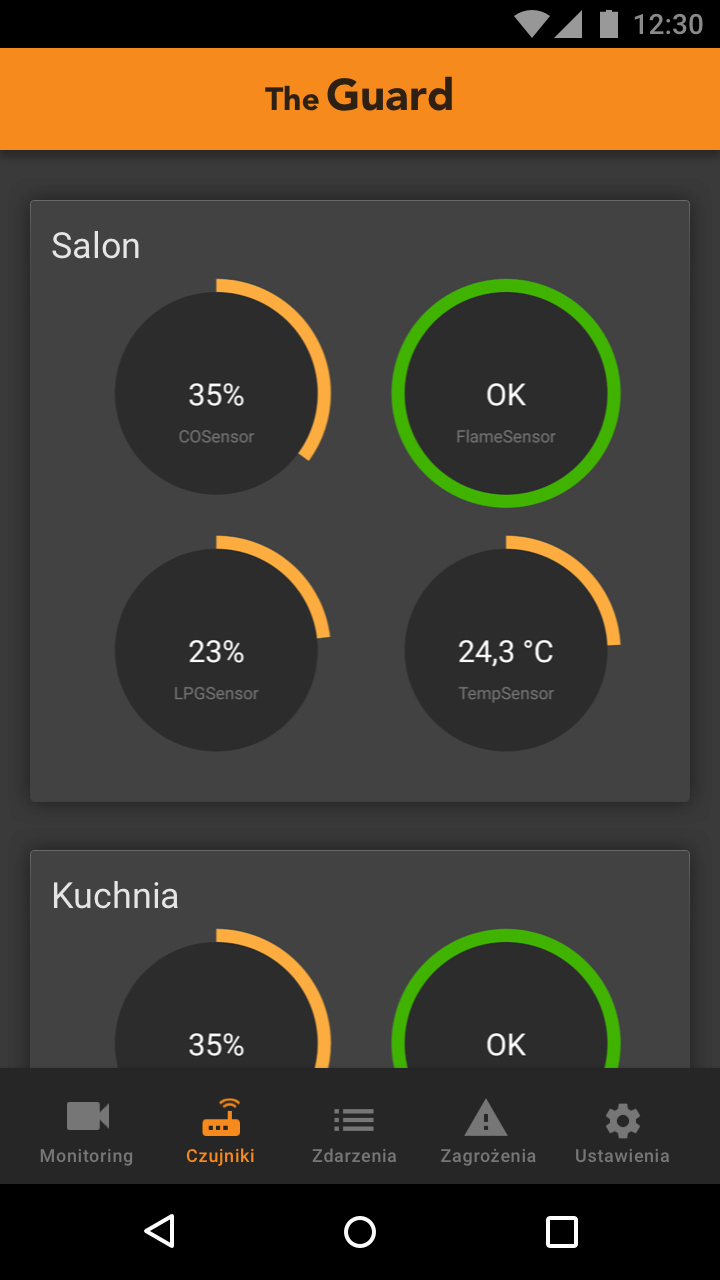
\includegraphics[height=5cm]{android-screenshots/Czujniki.png}}
    \hfill
    \subfloat[Aplikacja iOS]{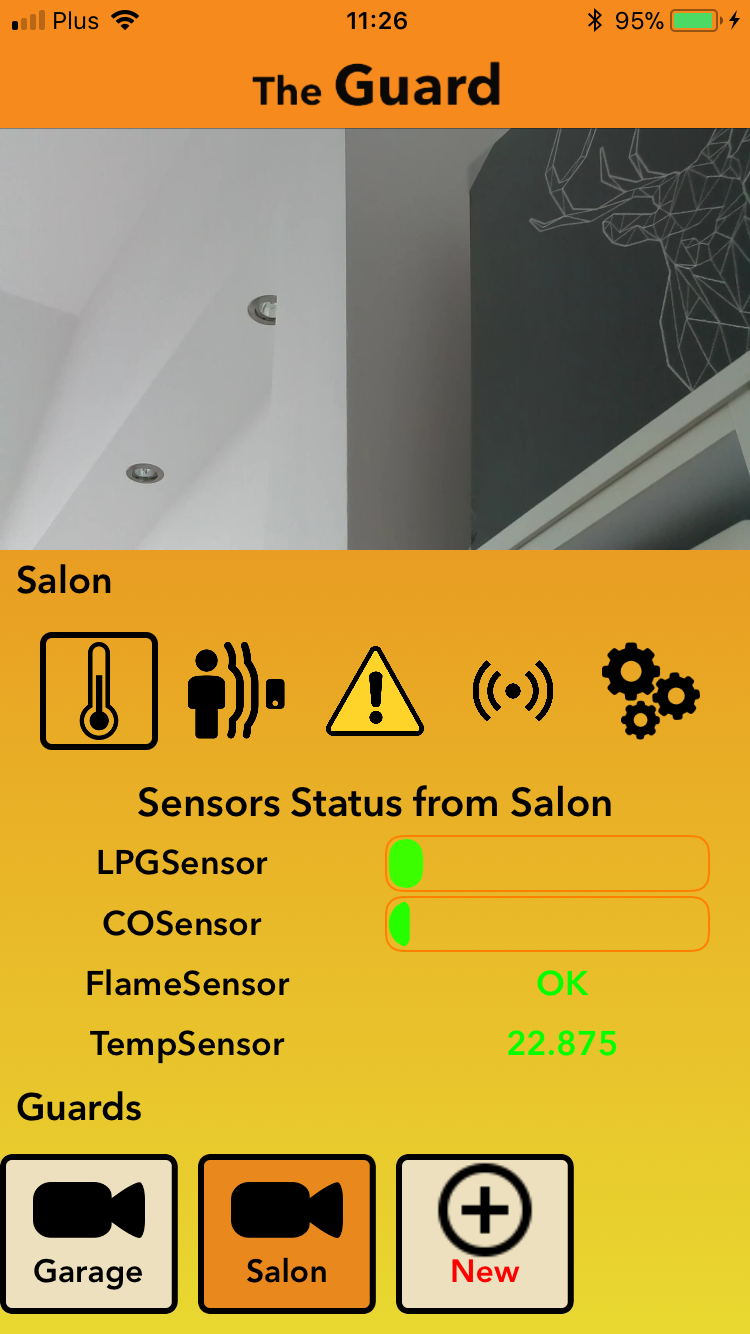
\includegraphics[height=5cm]{ios_screenshots/sensors.png}}
    \hfill
    \subfloat[Aplikacja webowa]{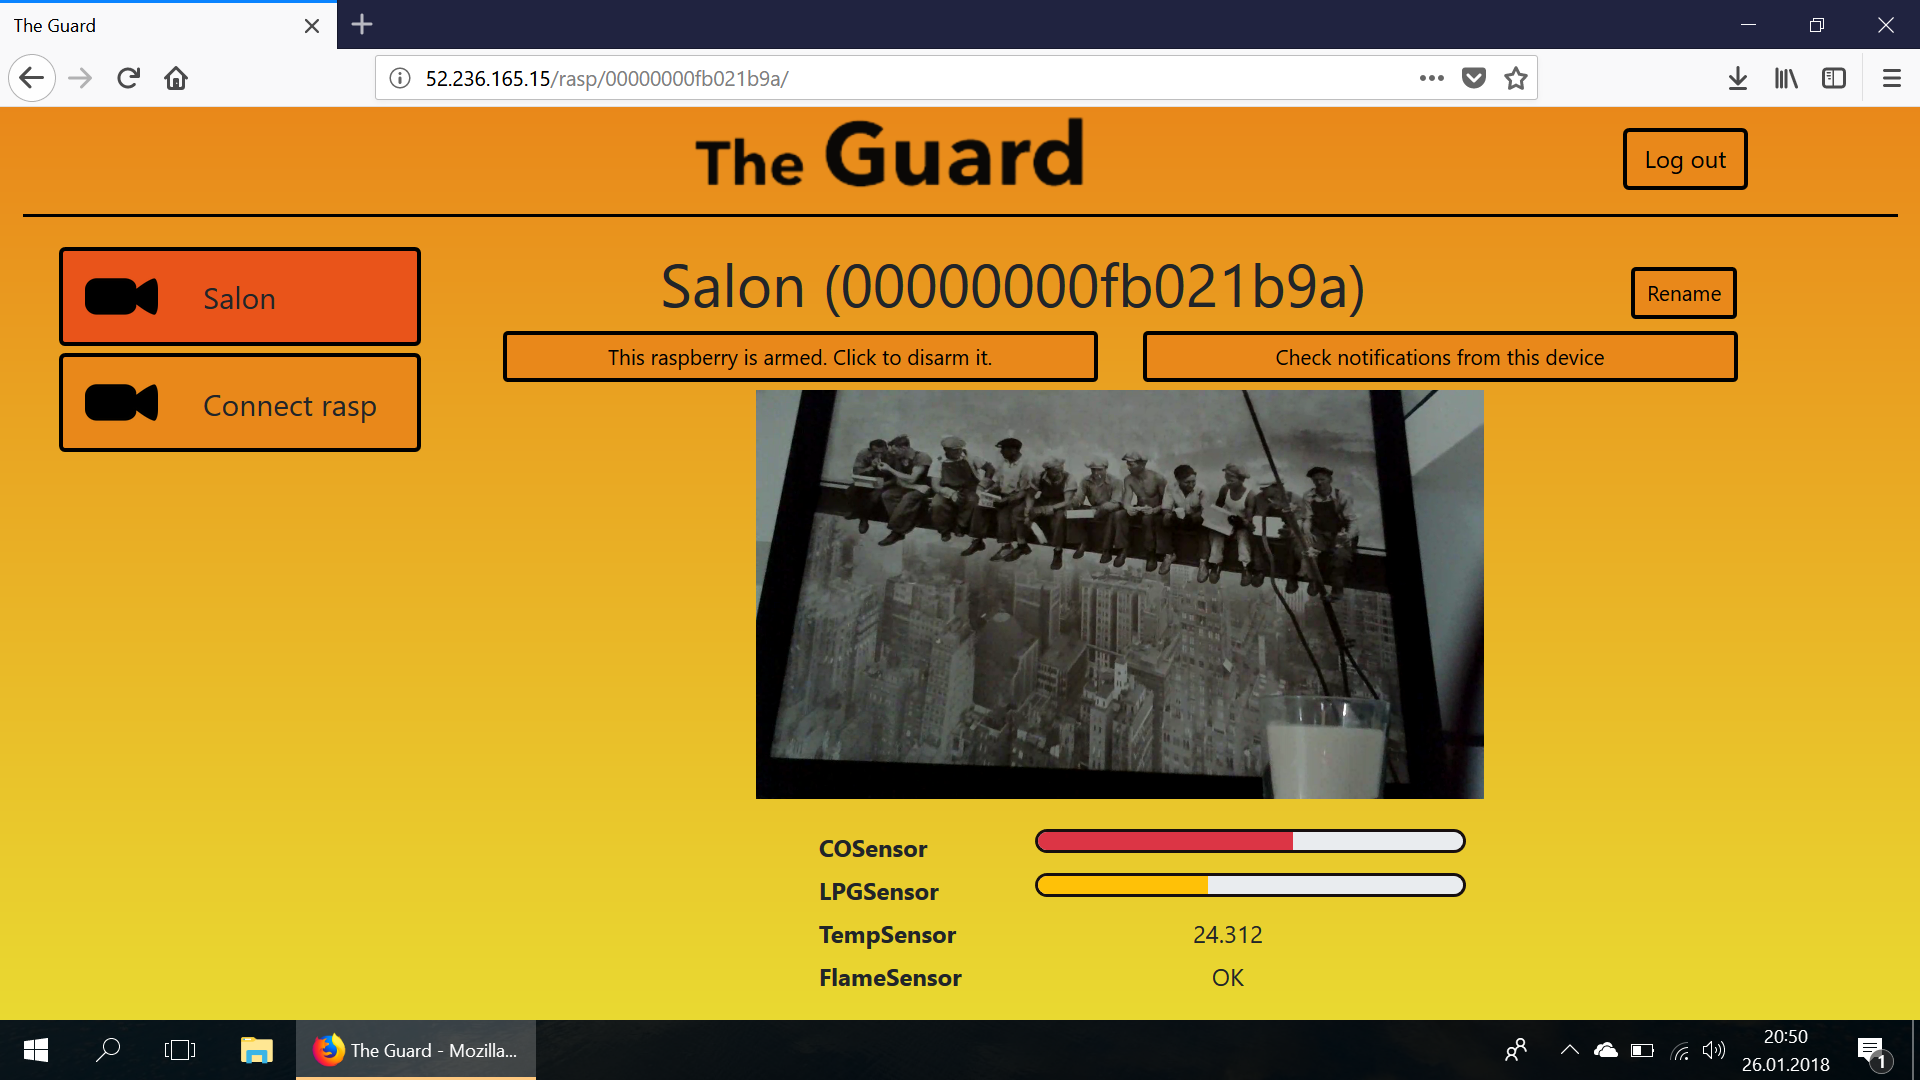
\includegraphics[height=4cm]{web_screenshots/rasp_view.png}}
    \caption{Widok czujników}
    \label{fig:czujniki}
\end{figure}

\paragraph{Dziennik zdarzeń}
W tej sekcji użytkownik ma dostęp do historii zdarzeń w systemie.
\nopagebreak
\begin{figure}[H]
    \centering
    \subfloat[Aplikacja Android]{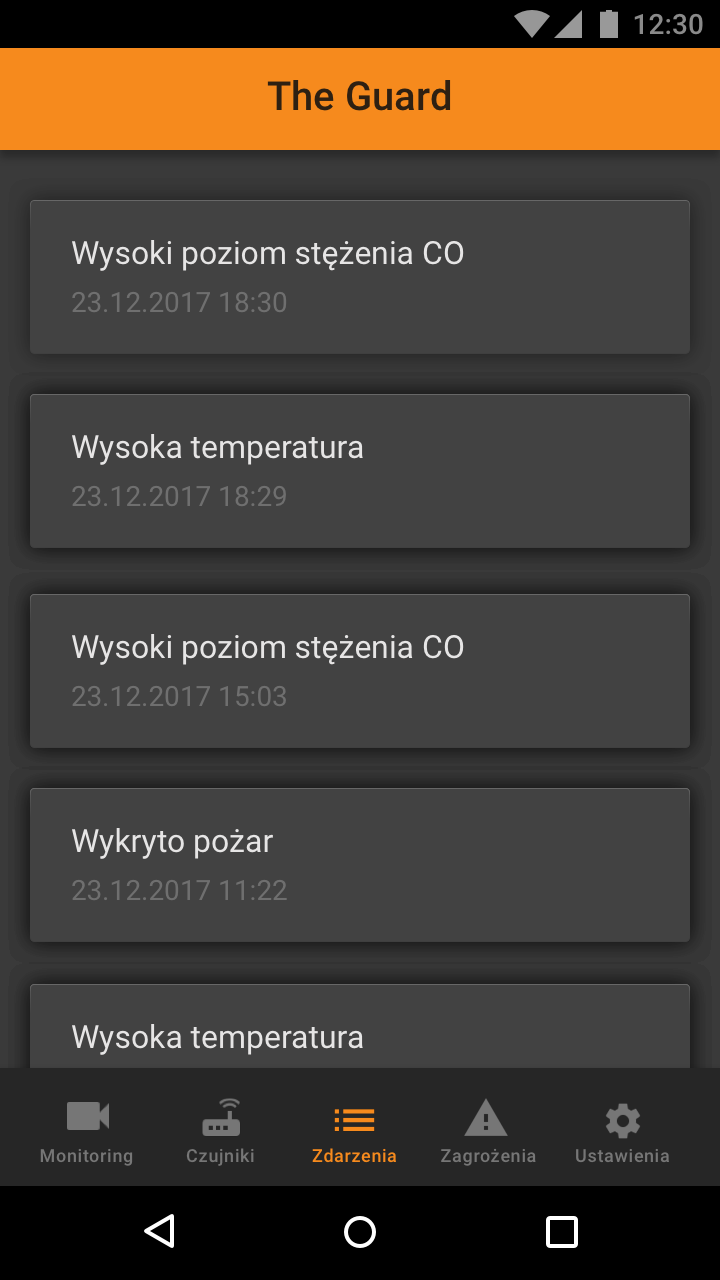
\includegraphics[height=5cm]{android-screenshots/Zdarzenia.png}}
    \hfill
    \subfloat[Aplikacja iOS]{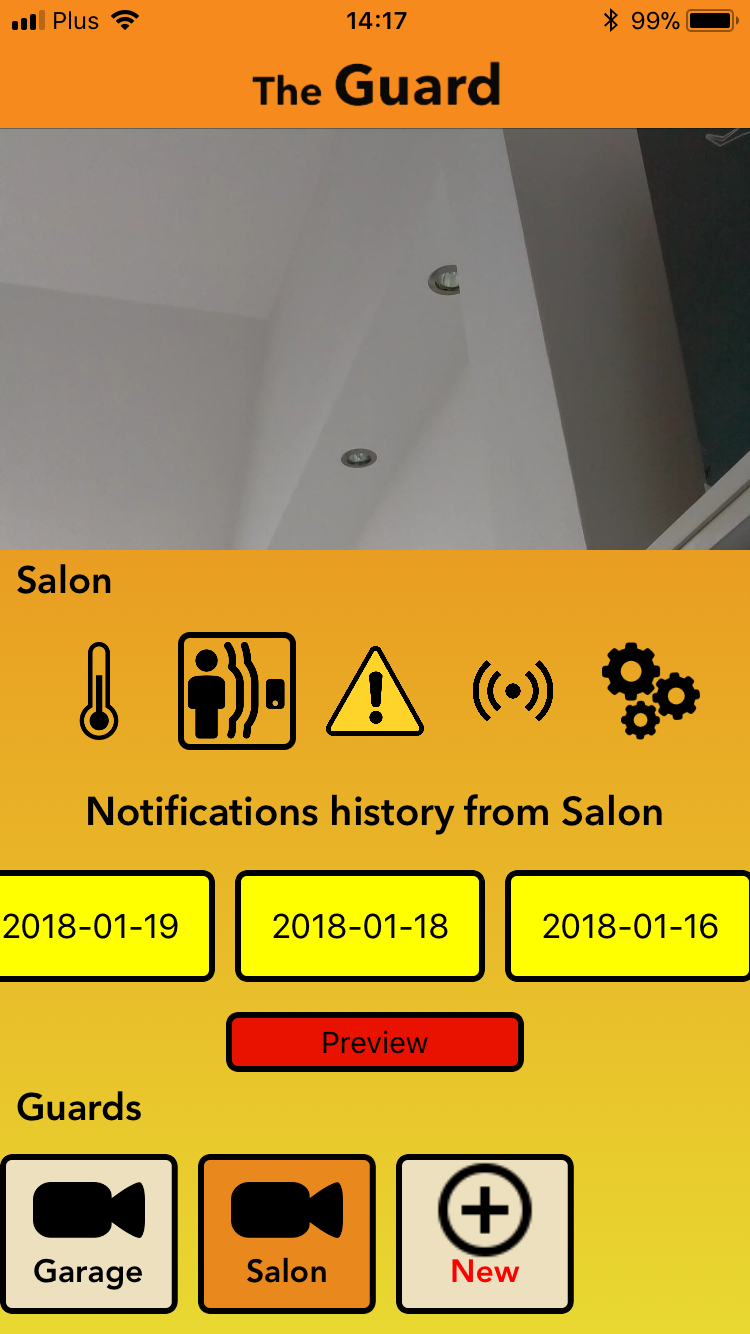
\includegraphics[height=5cm]{ios_screenshots/history.png}}
    \hfill
    \subfloat[Aplikacja webowa]{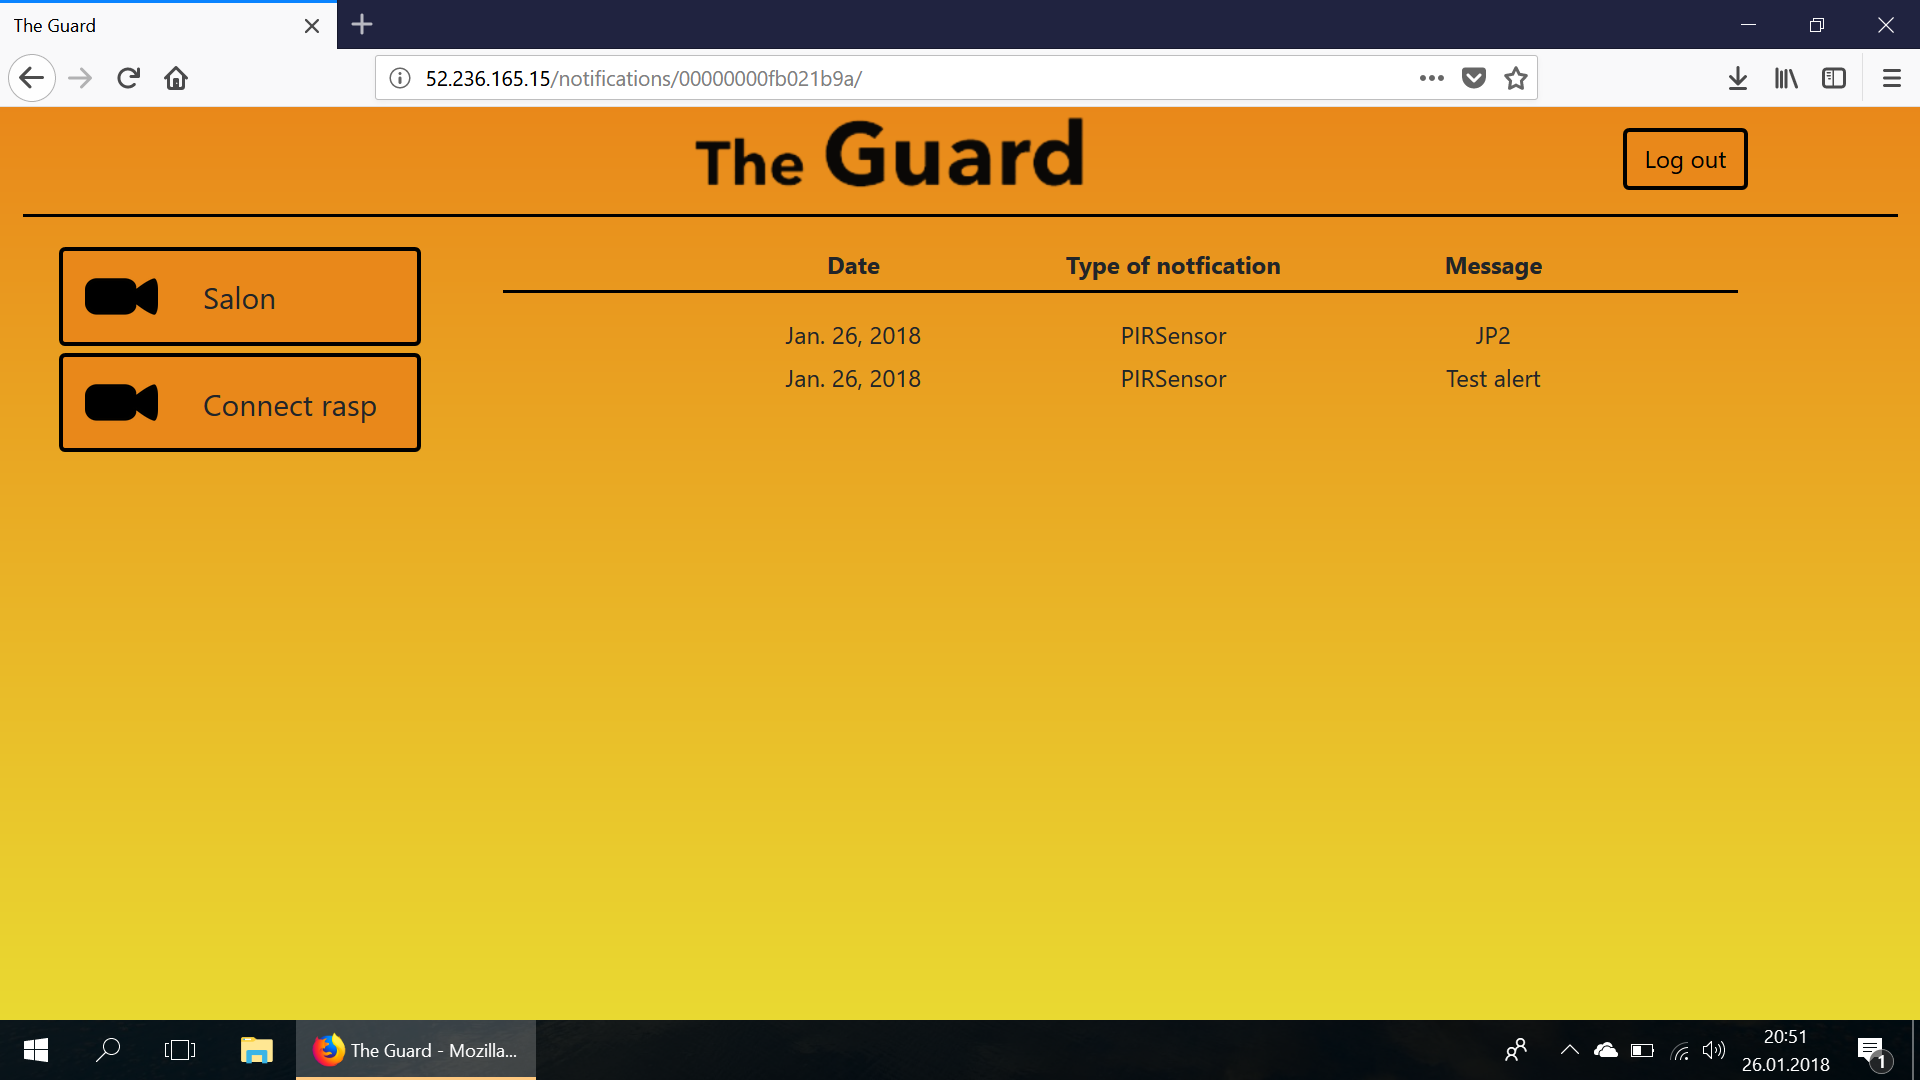
\includegraphics[height=4cm]{web_screenshots/rasp_notifications2.png}}
    \caption{Widok zdarzeń}
    \label{fig:zdarzenia}
\end{figure}

\paragraph{Ostatnie zagrożenia}
Prezentacja ostatniego nagranego zagrożenia. Służy do szybkiego przeglądu ostatniego niebezpieczeństwa i prezentuje ostatni nagrany materiał video.
\nopagebreak
\begin{figure}[H]
    \centering
    \subfloat[Aplikacja Android]{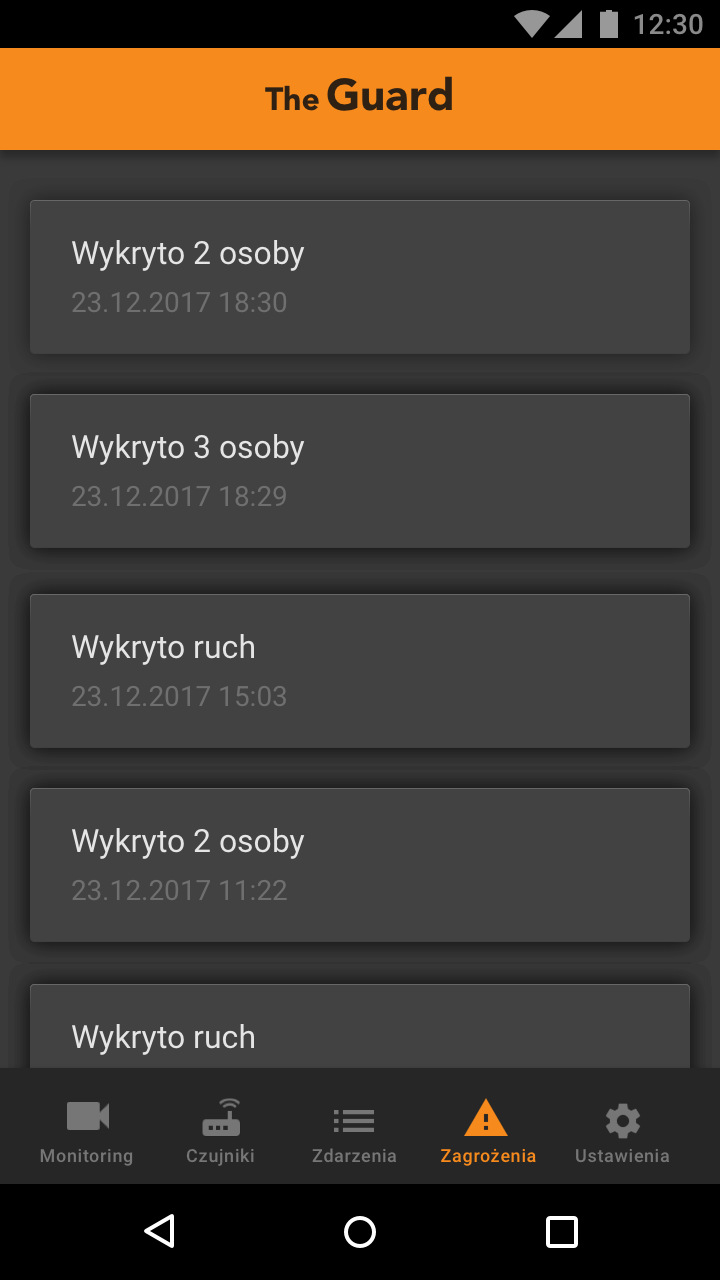
\includegraphics[height=5cm]{android-screenshots/Zagrozenia.png}}
    \hfill
    \subfloat[Aplikacja iOS]{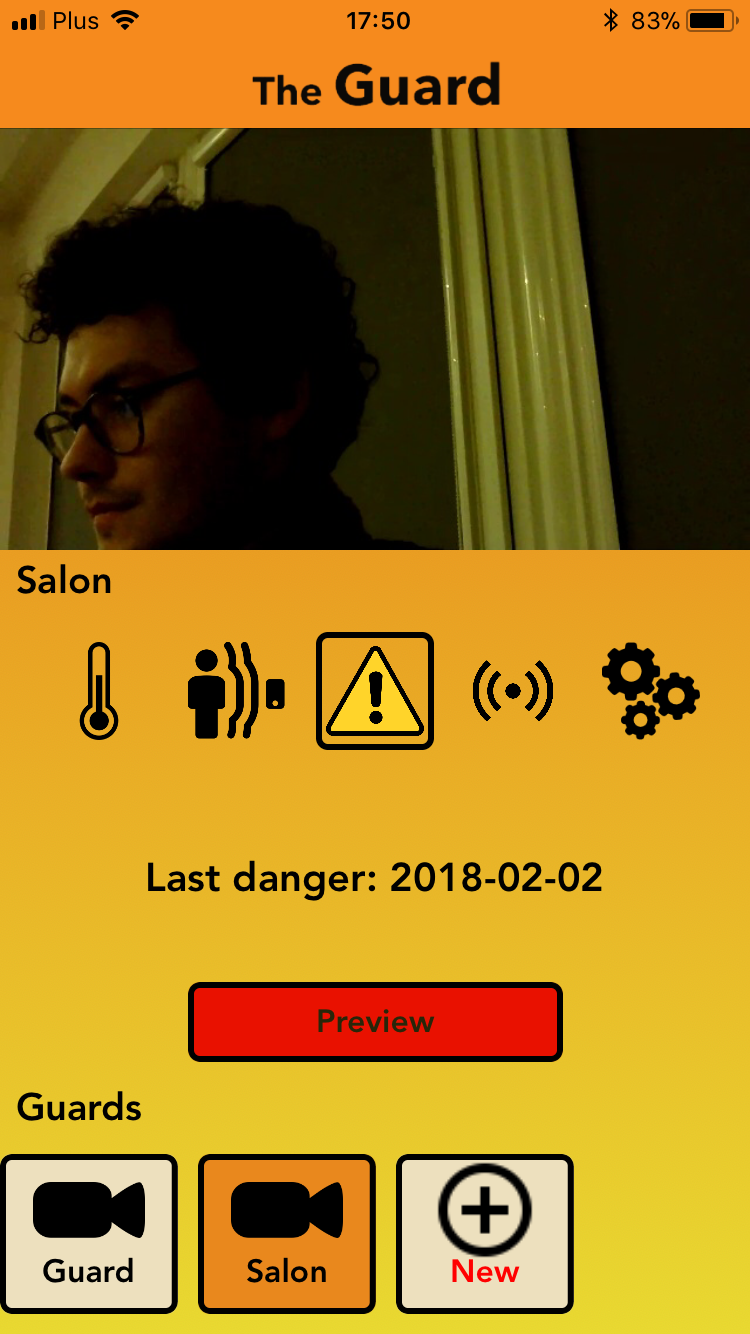
\includegraphics[height=5cm]{ios_screenshots/dangeriOS.png}}
    \hfill
    \subfloat[Aplikacja webowa]{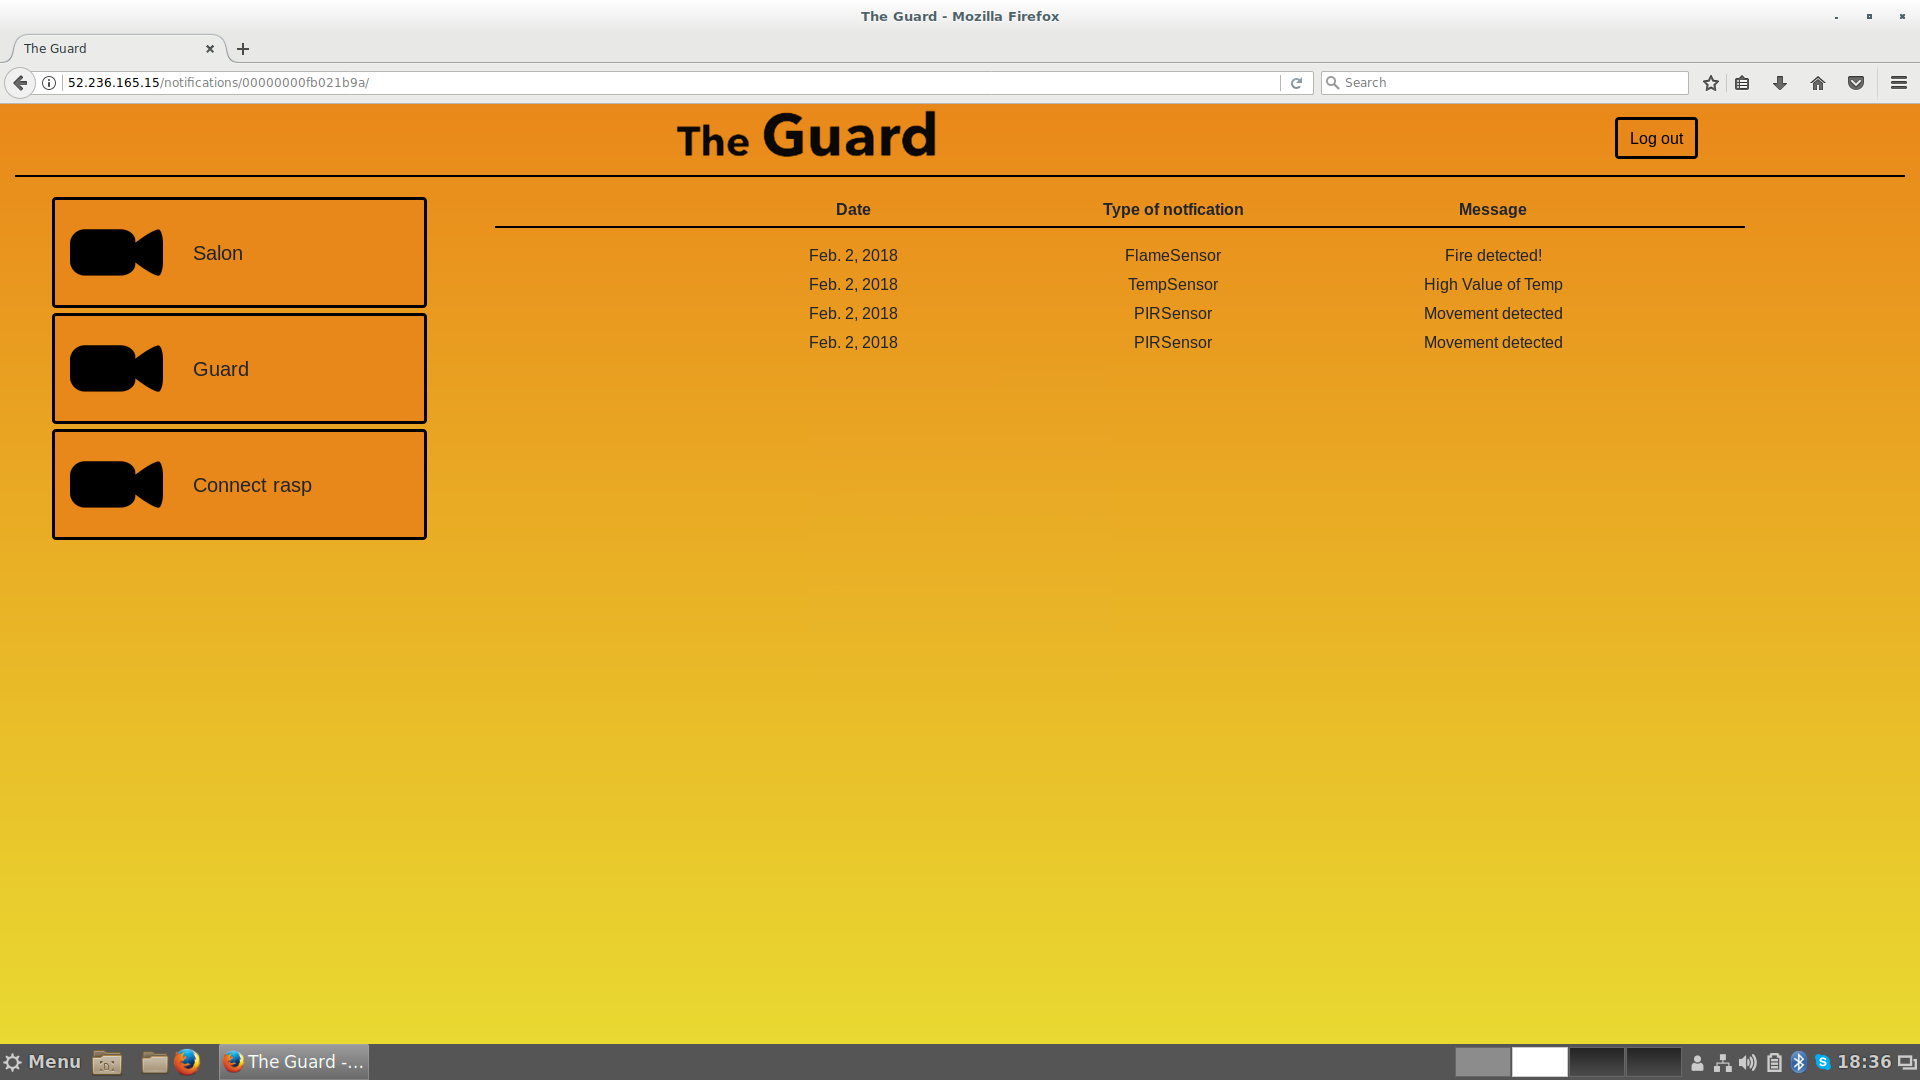
\includegraphics[height=4cm]{web_screenshots/rasp_notifications.png}}
    \caption{Widok zagrożeń}
    \label{fig:zagrozenia}
\end{figure}
\pagebreak

\paragraph{Ustawienia urządzenia}
Użytkownik ma możliwość zmiany nazwy urządzenia, które zazwyczaj reprezentuje miejsce, w którym się znajduje. Istnieje również możliwość uzbrojenia i wyłączenia każdego urządzenia. Sprowadza się to do tego, że w przypadku zaznaczenia opcji "Disarmed"  użytkownik nie otrzyma kolejnych notyfikacji o zagrożeniach. Opcja ta może okazać się przydatna w momencie uszkodzenia któregoś z modułów i tym samym błędnych danych wysyłanych z czujników.
\nopagebreak
\begin{figure}[H]
    \centering
    \subfloat[Aplikacja Android]{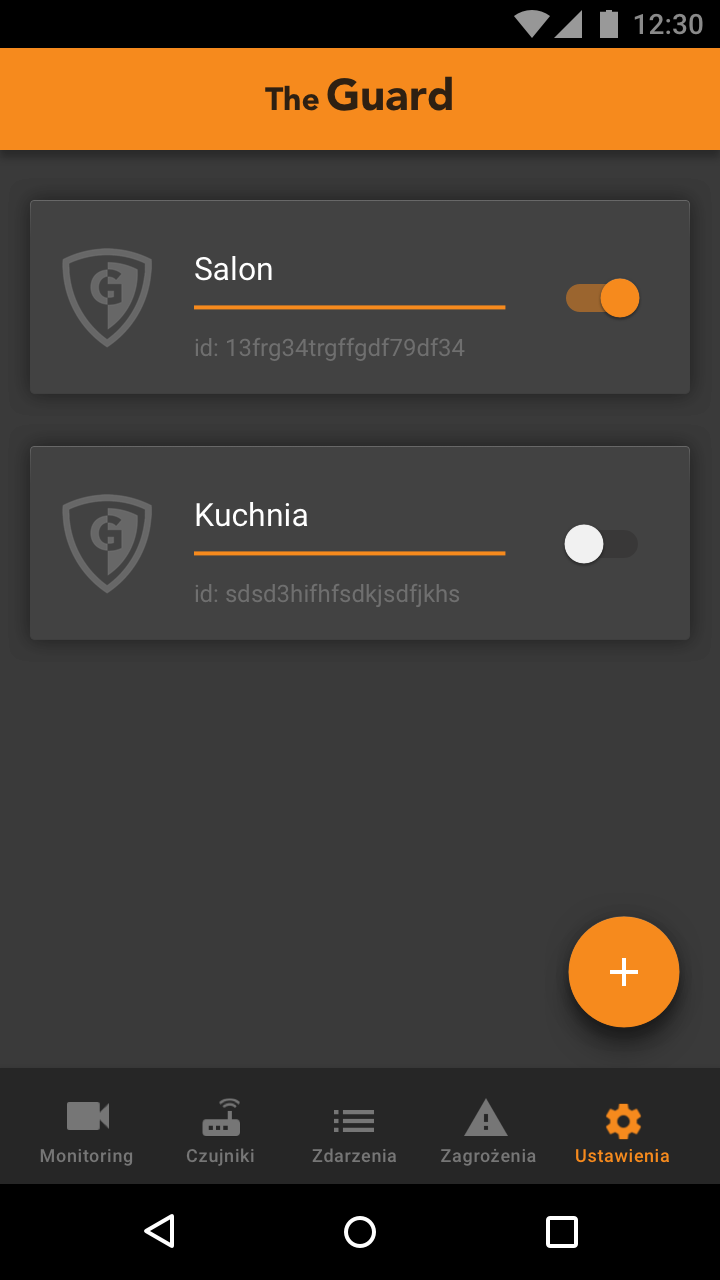
\includegraphics[height=5cm]{android-screenshots/Ustawienia.png}}
    \hfill
    \subfloat[Aplikacja iOS]{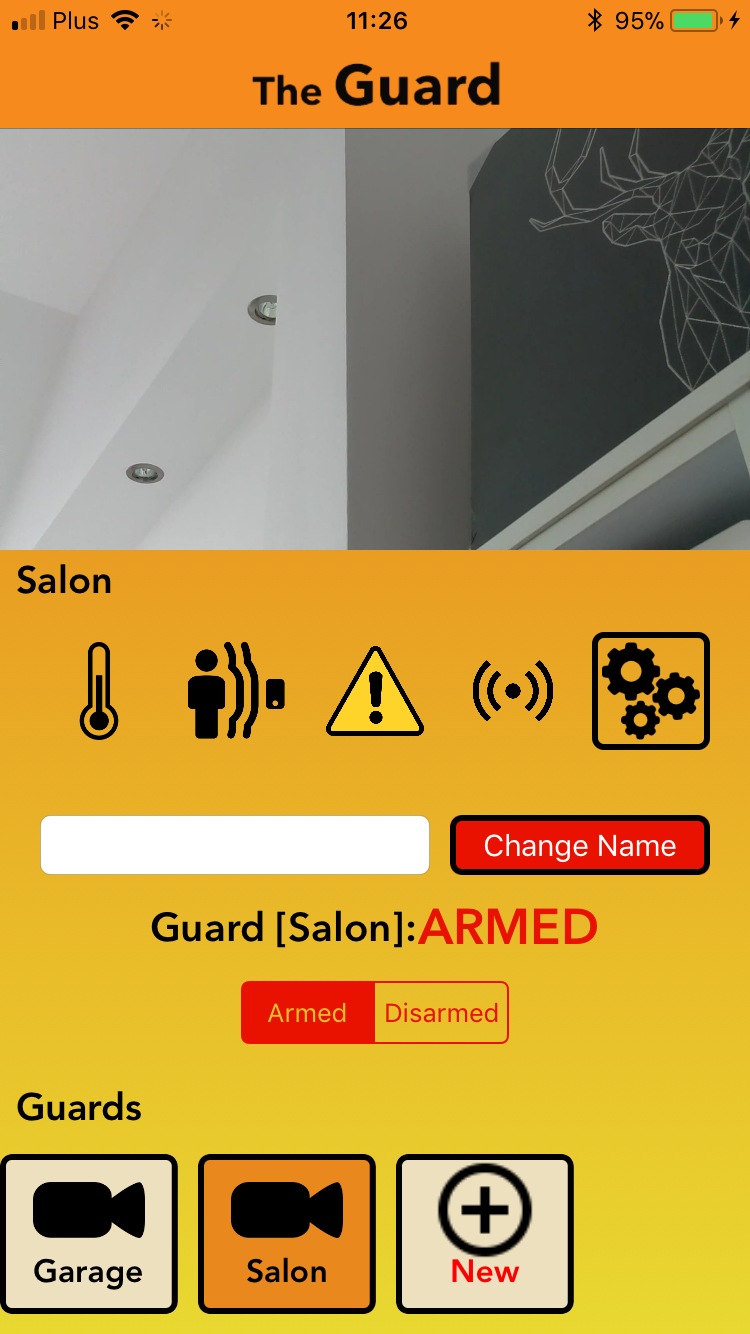
\includegraphics[height=5cm]{ios_screenshots/settings.png}}
    \hfill
    \subfloat[Aplikacja webowa]{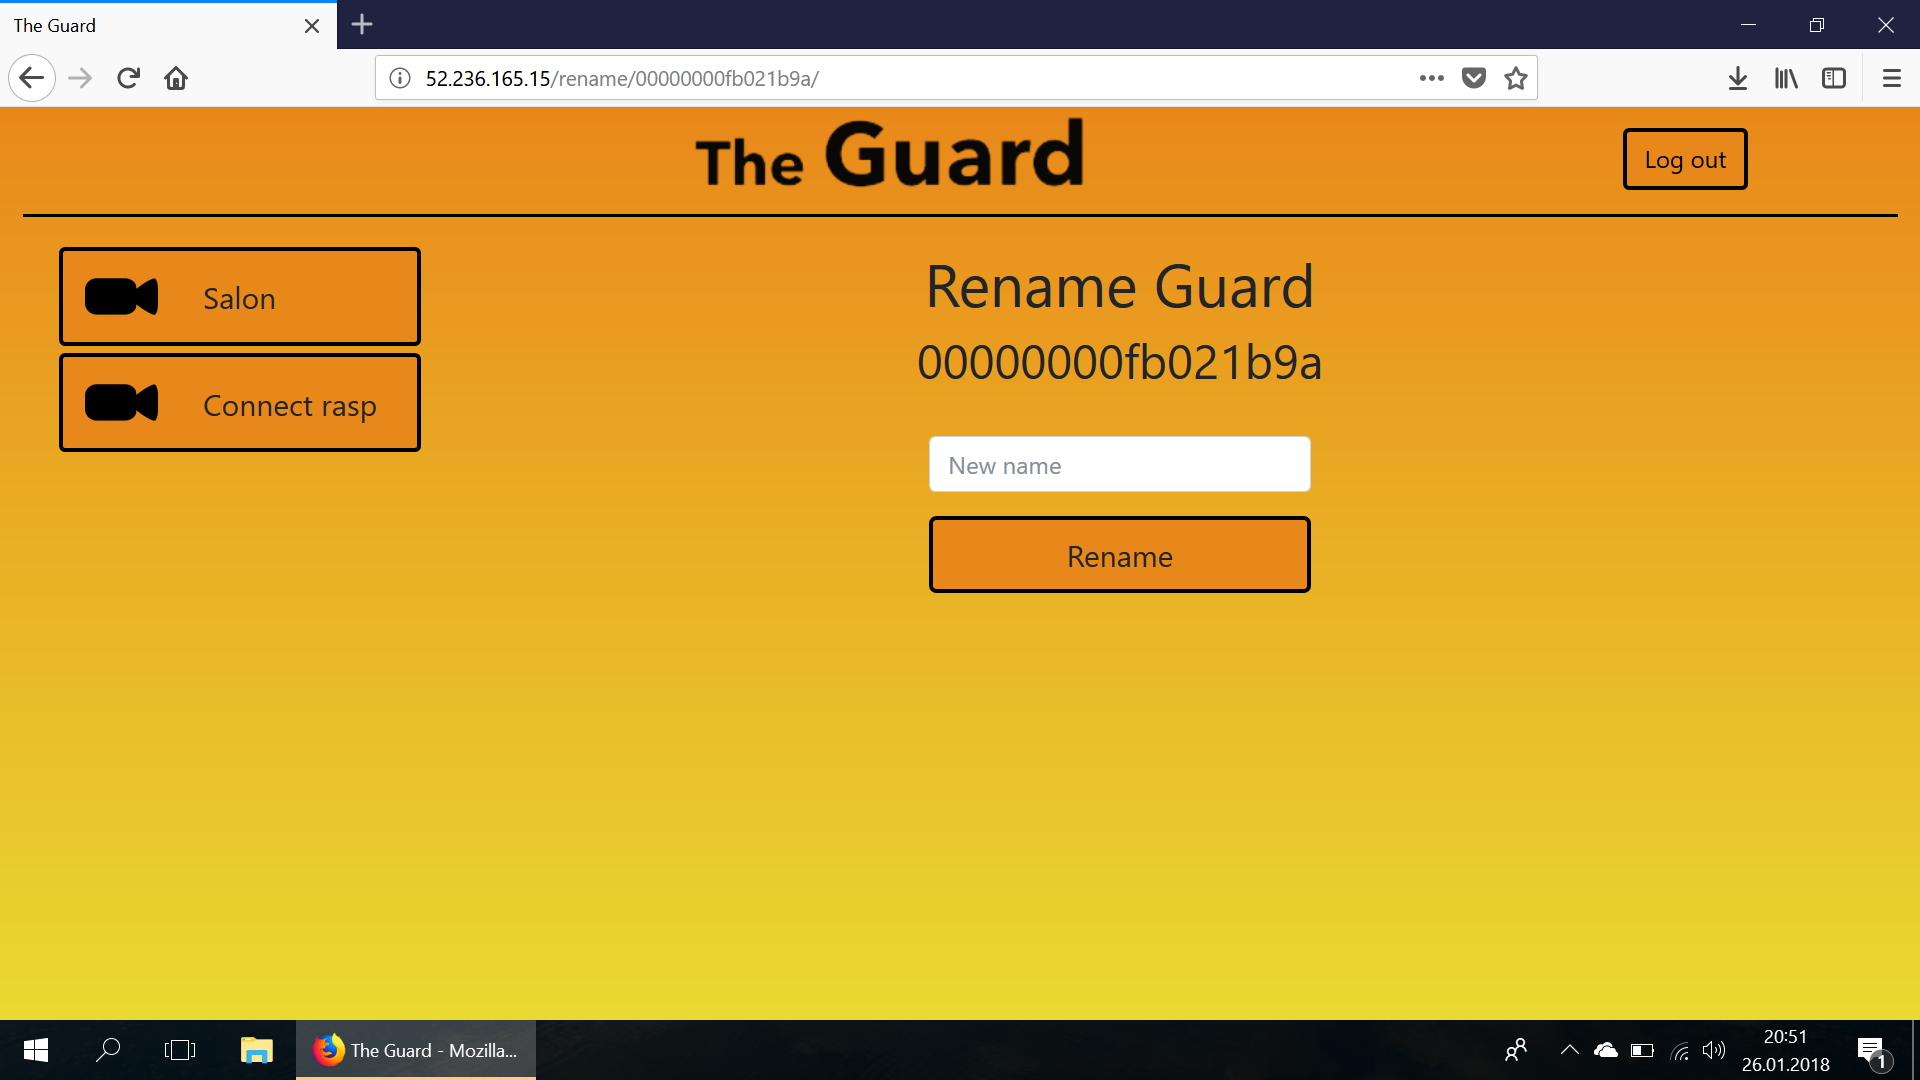
\includegraphics[height=4cm]{web_screenshots/rasp_rename.png}}
    \caption{Widok ustawień}
    \label{fig:ustawienia}
\end{figure}

\section{Aplikacja Android}
\subsection{Wybór narzędzi}
Do stworzenia aplikacji mobilnej na system Android użyto języka Kotlin - języka stworzonego przez firmę JetBrains, który 17 maja 2017 roku został uznany przez Google jako oficjalny język programowania aplikacji na platformę Android.\footnote{\url{https://twitter.com/Android/status/864911929143197696}}
Kotlin ściśle współegzystuje z kodem stworzonym w Javie i w przypadku Androida jest kompilowany do kodu JVM.

Skorzystano ze środowiska Android Studio w wersji 3.0.1, do automatyzacji budowy projektu został wykrozystany Gradle w wersji 4.1.

Aplikacja skierowana jest na urządzenia z systemem Android od wersji Lollipop 5.0 (o numerze SDK większym niż 20), który został wydany 12.12.2014 r. Ograniczenie wersji spowodowane jest możliwością użycia bardziej zaawansowanych komponentów, niedostępnych dla niższych wersji. W styczniu 2018 r. oficjalne statystyki informują o tym, że około 80,7 \% wszystkich urządzeń z systemem Android na świecie ma wersję 5.0 lub wyższą.

\subsection{Architektura}
Aplikacja The Guard dla systemu Android została stworzona zgodnie z założeniami architektury Model View Presenter.
Architektura MVP zakłada rozdzielenie kodu źródłowego aplikacji na 3 kategorie:
\begin{itemize}
\item Model - kod odpowiedzialny za logikę biznesową, połączenie z serwerem i złożone operacje biznesowe,
\item View - kod odpowiedzialny wyłącznie za poprawne wyświetlanie przygotowanych informacji,
\item Presenter - kod odpowiedzialny za przygotowanie informacji otrzymanych z warstwy model do wyświetlenia w warstwie View.
\end{itemize}
Największą zaletą architektury MVP jest możliwość wygodnego testowania logiki aplikacji (w warstwie Presenter) oraz zastosowanie programowania reaktywnego przy użyciu biblioteki RxKotlin.
Warstwy komunikują się między sobą w sposób reaktywny - przy użyciu strumieni wydarzeń. Przykładowo klasa warstwy Presenter odpowiedzialna za wyświetlanie obrazu z kamery wykorzystuje klasę warstwy Model do asynchronicznej komunikacji z API.

\begin{figure}[H]
    \centering
    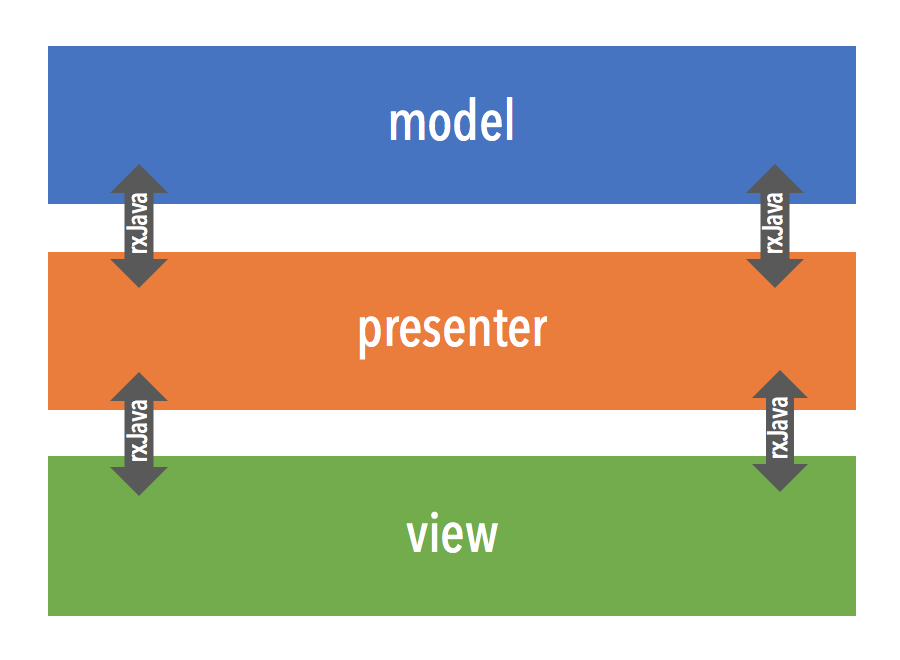
\includegraphics[width=9cm]{android-mvp.png}
    \caption{Struktura MVP [źródło własne]}
\end{figure}

\subsection{Interfejs użytkownika}
Aplikacja została zaprojektowana zgodnie z wytycznymi Material Design\footnote{Learning Material Design: Master Material Design and create beautiful, animated interfaces for mobile and web applications, Kyle Mew, Packt Publishing 2015}.
Do nawigacji po funkcjach aplikacji służy panel na dole ekranu - "Bottom Bar".
Zanim będzie on widoczny, użytkownik musi najpierw zalogować się (lub zarejestrować) przy użyciu adresu email oraz hasła.

\subsection{Wykorzystane biblioteki}
\begin{itemize}
    \item \textbf{com.squareup.retrofit2} - biblioteka służąca do wygodnej komunikacji z API
    \item \textbf{io.reactivex:rxandroid} - biblioteka zapewniająca \textit{Scheduler} platformy Android dla kodu reaktywnego,
    \item \textbf{com.jakewharton.rxbinding} - biblioteka zapewniająca nakładki na widoki Androida generujące zdarzenia dla programowania reaktywnego,
    \item \textbf{com.github.zurche:plain-pie} - biblioteka wyświetlająca diagramy na podstawie danych z czujników,
    \item \textbf{com.github.jacek-marchwicki.recyclerview-changes-detector} - biblioteka umożliwiająca automatyczną zmianę widoków po detekcji zmiany zbioru wyświetlanych danych,
    \item \textbf{com.google.code.gson} - biblioteka umożliwiająca serializacje i deserializacje obiektów
    \item \textbf{com.google.firebase} - biblioteki służące do obsługi usług Firebase
\end{itemize}

\subsection{}
CDane te trafiają do usługi \textit{Firebase Authentication}, która w przypadku pomyślnego logowania zwraca jego identyfikator.

\section{Aplikacja iOS}
Aplikacja przeznaczona jest na urządzenia z systemem operacyjnym iOS od wersji 10.0. 
Nie wspiera ona wcześniejszych wersji ze względu na nowe funkcje, które Apple wprowadziło wraz z pojawieniem się iOS 10.0 (m.in. klasa UNUserNotificationCenter). Jednak 93\% wszystkich obecnych użytkowników tego systemu(rys. 5.1) jest w stanie zainstalować oprogramowanie a liczba ta stale rośnie. Aplikacja wspiera zarówno telefony komórkowe iPhone jak i tablety iPad. 
\begin{figure}[ht]
	\centering
	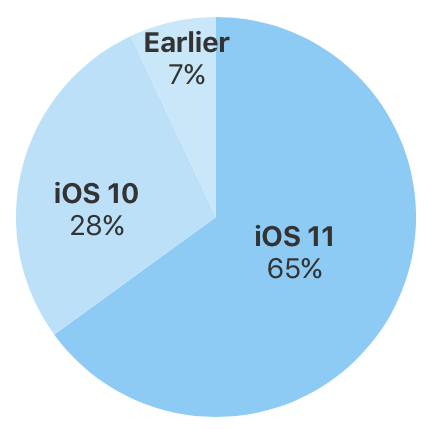
\includegraphics[width=4cm]{ios_screenshots/iOSstat.png}
	\caption{Udziały wersji systemu iOS z 18.01.2018 \protect\cite{iosversions}}
\end{figure}
Napisana w stosunkowo nowym języku Swift (zaprezentowany przez Apple w 2014 roku) w oparciu o architekturę MVC (Model-View-Controller) wykorzystując przy tym programowanie reaktywne i funkcjonalne. Aplikacja powstała w programie Xcode. Programowanie reaktywne zrealizowano przy pomocy biblioteki RxSwift. Ten paradygmat programowania związany jest z pojęciem obserwatora i sekwencji obserwowalnych. Każdy obserwator wywołując funkcję 'subscribe' na elemencie obserwowalnym otrzymuje informację o każdej zmianie na tym obiekcie. RxSwift wykorzystano m.in w celu wznowienia streamu obrazu z kamery w momencie przejścia aplikacji z trybu pracy w tle do trybu aktywnego. Oznacza to, że po wyjściu z aplikacji i po ponownym jej uruchomieniu tracono obraz ze streamu. Przyczyną jest polityka Apple, która nie zaleca aby aplikacje pracowały w tle i domyślnie wyłącza każdą taką aktywność. Ma to na celu przedłużenie żywotności baterii i optymalizacji całego systemu poprzez ograniczenie ilości zajmowanych zasobów \cite{backgroundmodes}.  Oczywiście istnieje możliwość włączenia pracy w tle, jednakże konieczne jest aktywowanie trybu "Background Modes" i zaznaczenie konkretnej aktywności, którą chcielibyśmy wykonywać. Lista dozwolonych czynności możliwych do realizacji jest jednak ograniczona (rys. 5.2). 
\begin{figure}[ht]
	\centering
	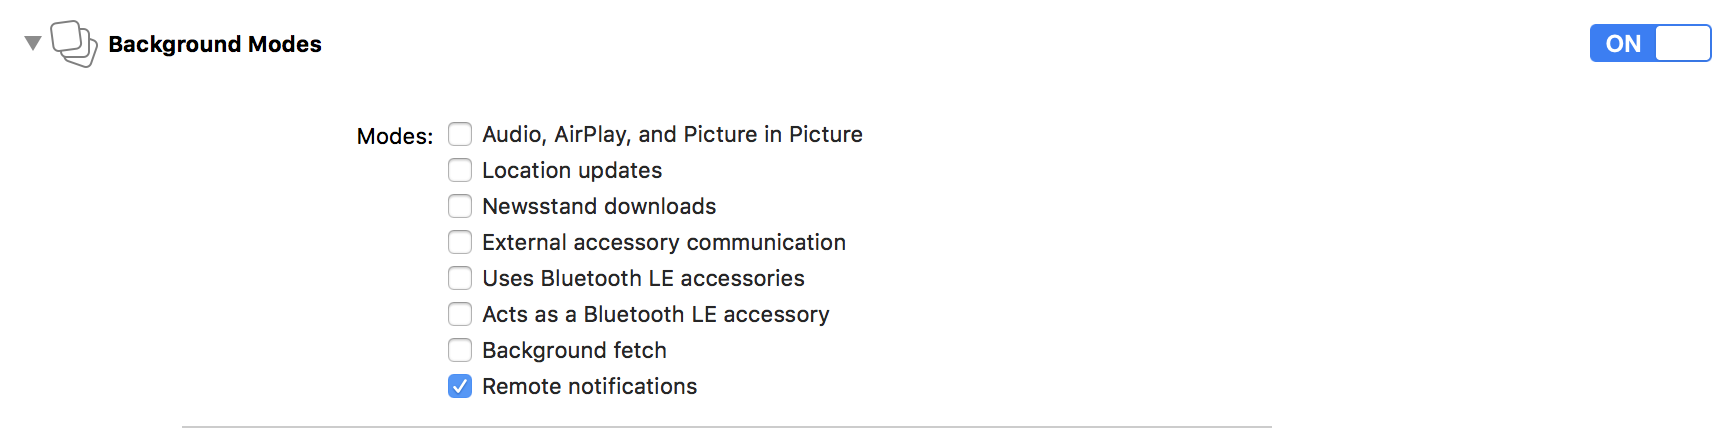
\includegraphics[width=10cm]{ios_screenshots/backgroundModes.png}
	\caption{Tryby pracy w tle [źródło własne]}
\end{figure}
Próba oszustwa i wykonywania innej pracy w tle niż zaznaczona zostanie wychwycona w procesie weryfikacji przed jej publikacją na platformie Apple Store. Dzięki programowaniu reaktywnemu problem wznowienia podglądu obrazu został rozwiązany co prezentuje poniższy kod:
\begin{verbatim}
let appDelegate = UIApplication.shared.delegate as! AppDelegate
        appDelegate.inBackground.asObservable().subscribe(onNext: { (value) in
            if let streamView = self.streamView {
                if let player = self.currentPlayer {
                    if value == false {
                        self.streamVideoFrom(urlString: self.currentUrlString!)
                        print("Enter foreground")
                    } else {
                        print("Enter background")
                        streamView.layer.sublayers?.forEach({ (layer) in
                            layer.removeFromSuperlayer()
                        })
                    }
                }
            }
        }).disposed(by: disposeBag)
\end{verbatim}
Zmienna 'inBackground', która jest zmienną obserwowalną, ustawiana jest w oddzielnej klasie AppDelegate (klasa, która zapewnie poprawną interakcję z systemem iOS) na wartość true w chwili przejścia do trybu pracy w tle i na wartość false w przeciwnym wypadku. Klasa, w której wywoływany jest funkcja 'subscribe' jest obserwatorem tej zmiennej. Kod wewnątrz funkcji subscribe uruchamiany jest przy każdej zmianie wartości 'inBackground' i wznawia ponownie stream po każdym ponownym uruchomieniu programu.
"Programowanie funkcjonalne natomiast polega na traktowaniu funkcji jako obiektu. Oznacza to, że mogą być one zapisywane, kopiowane i przekazywane tak samo jak wszystkie inne obiekty. Mogą być używane jako parametry innych funkcji." \cite[p.~172]{proswift}. Wykorzystane są w miejscach gdzie konieczne jest przekształcanie danych:
\begin{verbatim}
lastNotification = notifications.array.sorted(by: { (n1, n2) -> Bool in
	n1.date > n2.date 
}).filter({ (notif) -> Bool in return notif.type == "PIRSensor"}).first
\end{verbatim}
Na tablicy z notyfikacjami zastosowano szereg kolejnych funkcji: posortowano je malejąco według daty, przefiltrowano w taki sposób aby wybrać tylko te o typie 'PIRSensor' czyli te pochodzące z czujnika ruchu. Na sam koniec wybrano tylko jeden pierwszy element z wybranych i wynik wpisano do zmiennej lastNotification. Ważne jest, że każda kolejna wywoływana funkcja np. filter, odbiera wynik poprzedniej. 

Strukturę kodu (rys. 5.3) podzielono na kilka osobnych, logicznych części. Folder Firebase zawiera model bazy danych czujników, które zapisane są na serwerach Firebase. W folderze GuardManager znajdują się elementy odpowiedzialne za komunikację REST-ową z serwerem Django i modele bazy danych znajdującej się na naszym serwerze. Folder Views jest zbiorem widoków, które wczytywane są w zależności, w której sekcji się znajdujemy (opis sekcji niżej). ViewController.swift jest głównym kontrolerem zarządzającym widokami i modelami. Odpowiada za załadowanie odpowiedniego widoku i prezentację danych z odpowiedniej sekcji. W folderze GuardianAppTests napisane zostały testy jednostkowe, które sprawdzają poprawność przekształcania danych typu JSON (odpowiedź serwera) do obiektów zdefiniowanych w folderze GuardManager/Models. Klasy, których nazwy kończą się na Manager oznaczają obiekty typu Singleton. Celem takiego wzorca jest zapewnienie istnienia tylko jednej instancji w całej aplikacji i globalnego dostępu do tego obiektu. GuardManager, który odpowiada za pobieranie danych z bazy danych - taki obiekt nie powinien być utworzony więcej niż jeden raz, gdyż wszystkie klasy, które z niego korzystają nie potrzebują kolejnych instancji tej klasy. W ten sposób zapewniono, że zawsze odwołujemy się do tego samego obiektu.
\begin{figure}[ht]
	\centering
	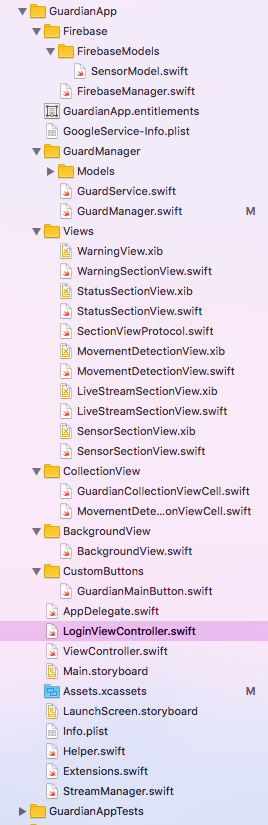
\includegraphics[width=4cm]{ios_screenshots/iOSstructure.png}
	\caption{Struktura aplikacji [źródło własne]}
\end{figure}
Instalacja zewnętrznych bibliotek odbywa się za pomocą CocoaPods. Jest to menadżer zależności dzięki któremu szybko możemy wyszukać i zainstalować wymagane oprogramowanie. Wszystkie użyte zależności przedstawiono poniżej: 
\begin{verbatim}
  pod 'Moya'
  pod 'MBProgressHUD', '~> 1.0'
  pod 'RxSwift',    '~> 4.0'
  pod 'RxCocoa',    '~> 4.0'
  pod 'IHKeyboardAvoiding'
  pod 'Moya-SwiftyJSONMapper'
  pod 'Firebase/Core'
  pod 'Firebase/Messaging'
  pod 'Firebase/Auth'
  pod 'Firebase/Database'
  pod 'M13ProgressSuite'
\end{verbatim}
Moya używana jest do asynchronicznej REST-owej komunikacji z serwerem Django. SwiftyJSONMapper przydatna okazuje się do przekształcenia odpowiedzi serwera w postaci JSON do wcześniej zdefiniowanego modelu. MBProgressHUD umożliwia wyświetlanie ekranu ładowania podczas pobierania informacji z serwera. RxSwift i RxCocoa to biblioteki do programowania reaktywnego. Moduły Firebas/Core itp. służą do komunikacji z serwerami Firebase. Ostatni 'pod M13ProgressSuite' służy do rysowania wykresów i animowanych elementów graficznych w systemie iOS.
Po uruchomieniu aplikacji pierwszym widokiem jest ekran logowania i rejestracji użytkowników (rys 5.4). 
\begin{figure}[ht]
	\centering
	
\includegraphics[width=5cm]{ios_screenshots/login.png}
	\caption{Ekran logowania [źródło własne]}
\end{figure}
Po prawidłowym uwierzytelnieniu użytkownika uzyskiwany jest dostęp do głównego widoku aplikacji. W górnej części możliwy jest wybór 5 sekcji:
sekcja czujników, sekcja historii notyfikacji, sekcja ostatnich zagrożeń przy wykryciu ruchu, sekcja monitoringu na żywo, sekcja ustawień. Wszystkie te sekcje dotyczą konkretnego urządzenia wybranego na pasku u dołu ekranu. Funkcje każdej z nich zostały opisane w rozdziale 6.1, tutaj zostaną zaprezentowane jedynie szczegóły implementacyjne i zrzuty ekranów z wersji na iOS. Przy pierwszym uruchomieniu nie istnieje żadne urządzenie przypisane do naszego konta użytkownika. Aby dodać pierwsze i kolejne stacje, od których chcemy otrzymywać notyfikacje o zagrożeniach a także śledzić i monitorować informacje z czujników należy wybrać przycisk "New" z plusikiem w dolnej części ekranu. Pojawi się okno z prośbą o wpisanie numeru identyfikującego urządzenie. Po chwili dodany "Guard" będzie widoczny w na liście.


\paragraph{Sekcja czujników:}
Jest to jedna z najważniejszych sekcji aplikacji (rys 5.5).  Otrzymuje ona dane z czujników w czasie rzeczywistym i prezentuje je użytkownikowi. Implementacja funkcjonalności prezentowania zagrożenia na konkretnym czujniku przy użyciu kolorów zrealizowana została przy pomocy modelu HSV, który w przeciwieństwie do RGB pozwala na bardzo proste przejście z jednego koloru do kolejnego poprzez zmienę tylko jednego parametru. Zmieniając parametr Hue zmieniamy barwę przy stałym nasyceniu i jasności. Wartość tego parametru równa 120\textdegree{} odpowiada kolorowi zielonemu, kolor czerwony to 0\textdegree{}. Przekształcając wartość otrzymaną z czujników, która jest z zakresu [0-1] na wartość z przedziału [120-0] otrzymano wspomniany efekt. 
Poniżej przedstawiono fragment konwersji danych z czujników na kolor w modelu HSV, gdzie zmienna sensors[0] reprezentuje czujnik LPG.
\begin{verbatim}
UIColor(hue: CGFloat(0.33 - (sensors[0].value * 0.33)),
saturation: 1, brightness: 1, alpha: 1)
\end{verbatim}
\begin{figure}[ht]
	\centering
	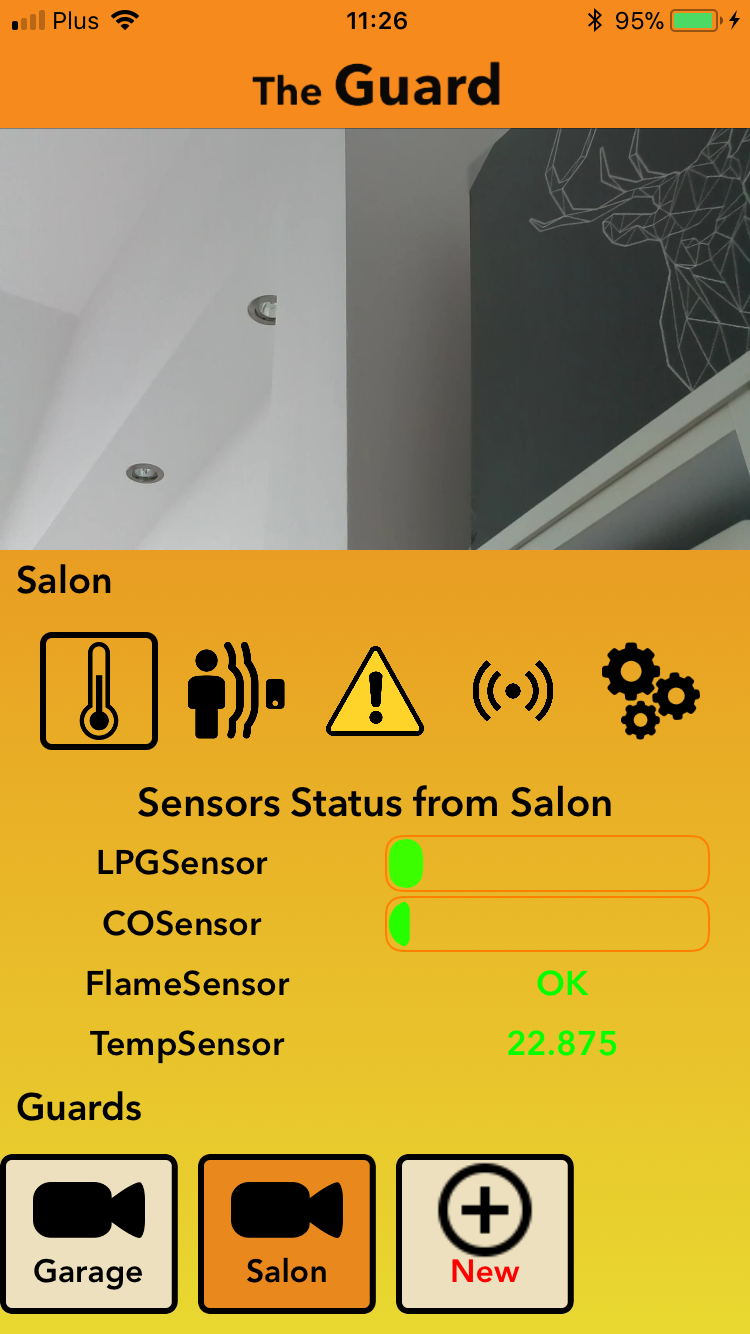
\includegraphics[width=5cm]{ios_screenshots/sensors.png}
	\caption{Sekcja czujników [źródło własne]}
\end{figure}
\paragraph{Sekcja historii notyfikacji:}
Po zaznaczeniu daty reprezentującej moment wystąpienia zagrożenia i wybraniu przycisku 'preview' prezentowana jest informacja o miejscu niebezpieczeństwa i jego rodzaju. (rys 5.6).
\begin{figure}[ht]
\centering
\begin{minipage}{.4\linewidth}
    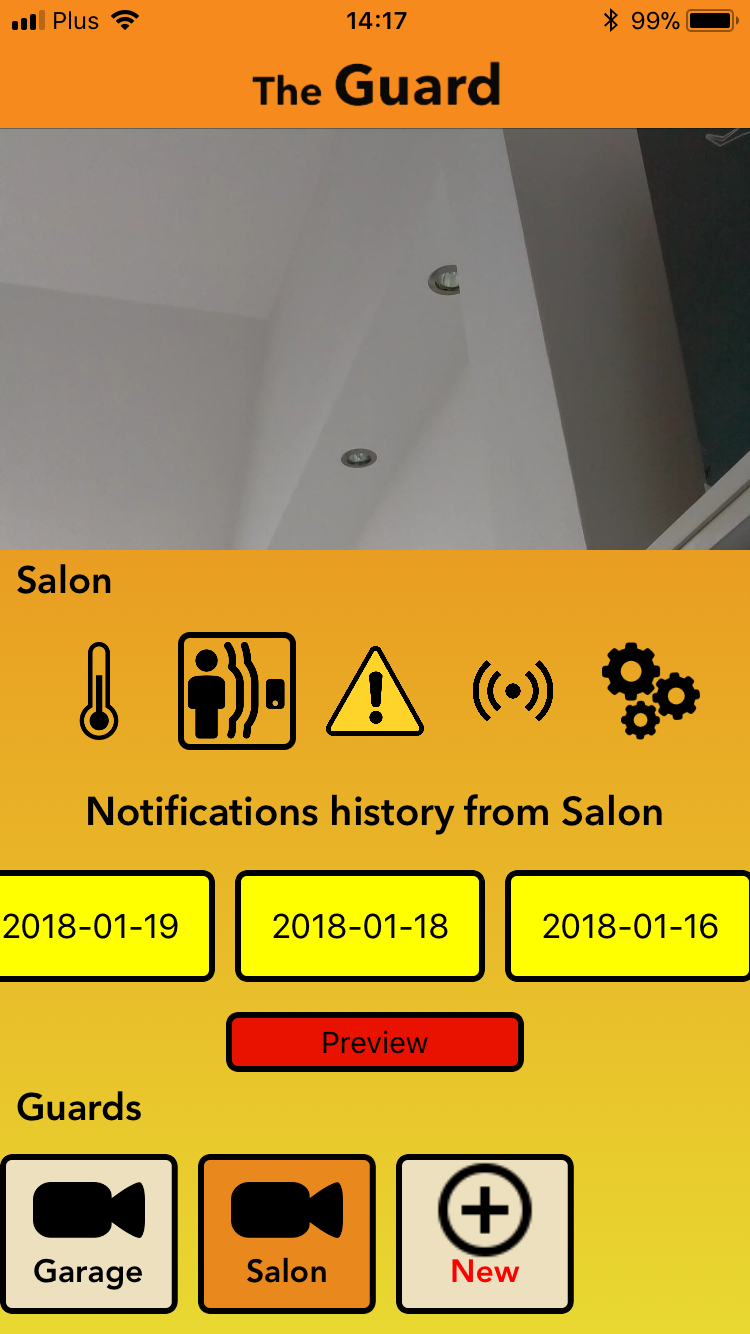
\includegraphics[width=\linewidth]{ios_screenshots/history.png}
    \caption{Sekcja historii notyfikacji  [źródło własne]}
    \label{img1}
\end{minipage}
\hspace{.05\linewidth}
\begin{minipage}{.4\linewidth}
    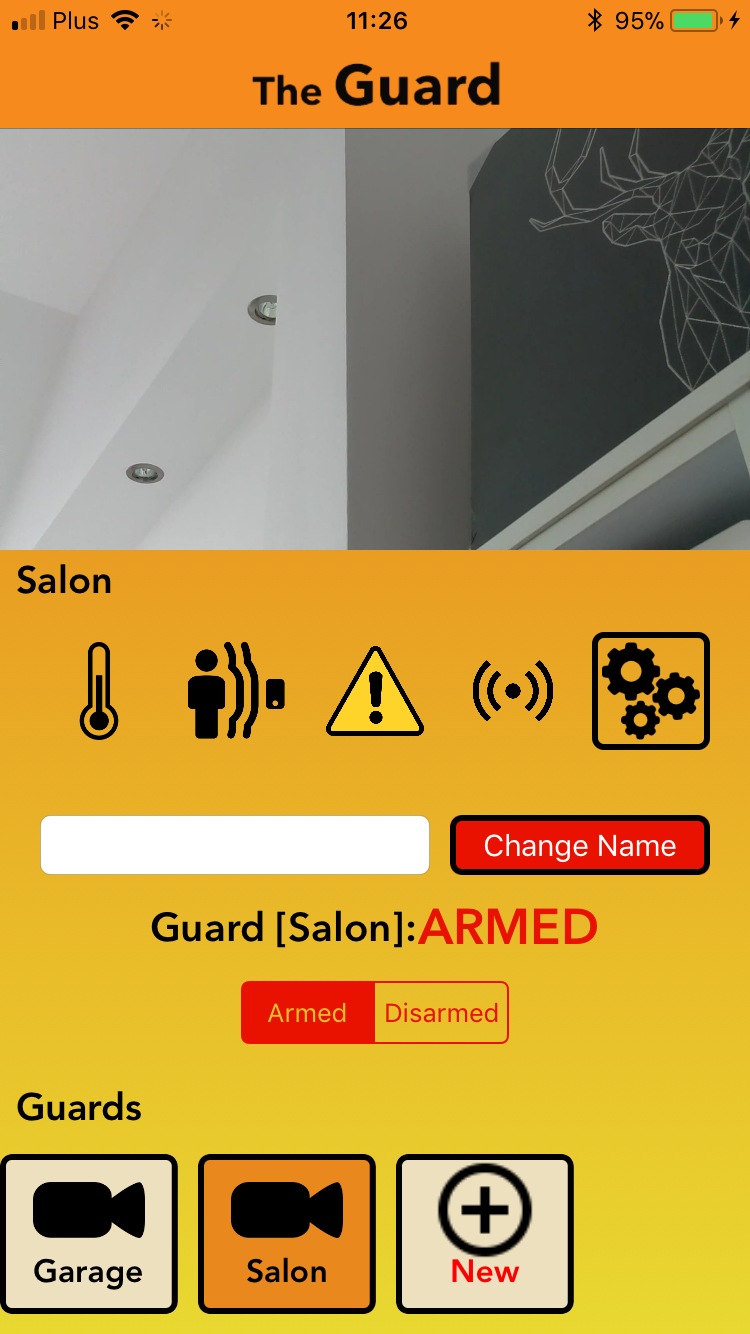
\includegraphics[width=\linewidth]{ios_screenshots/settings.png}
    \caption{Sekcja ustawień [źródło własne]}
    \label{img2}
\end{minipage}
\end{figure} 
\paragraph{Sekcja ustawień:}
Zrzut ekranu przedstawiono na rysunku (rys. x).
\begin{figure}[ht]
	\centering
	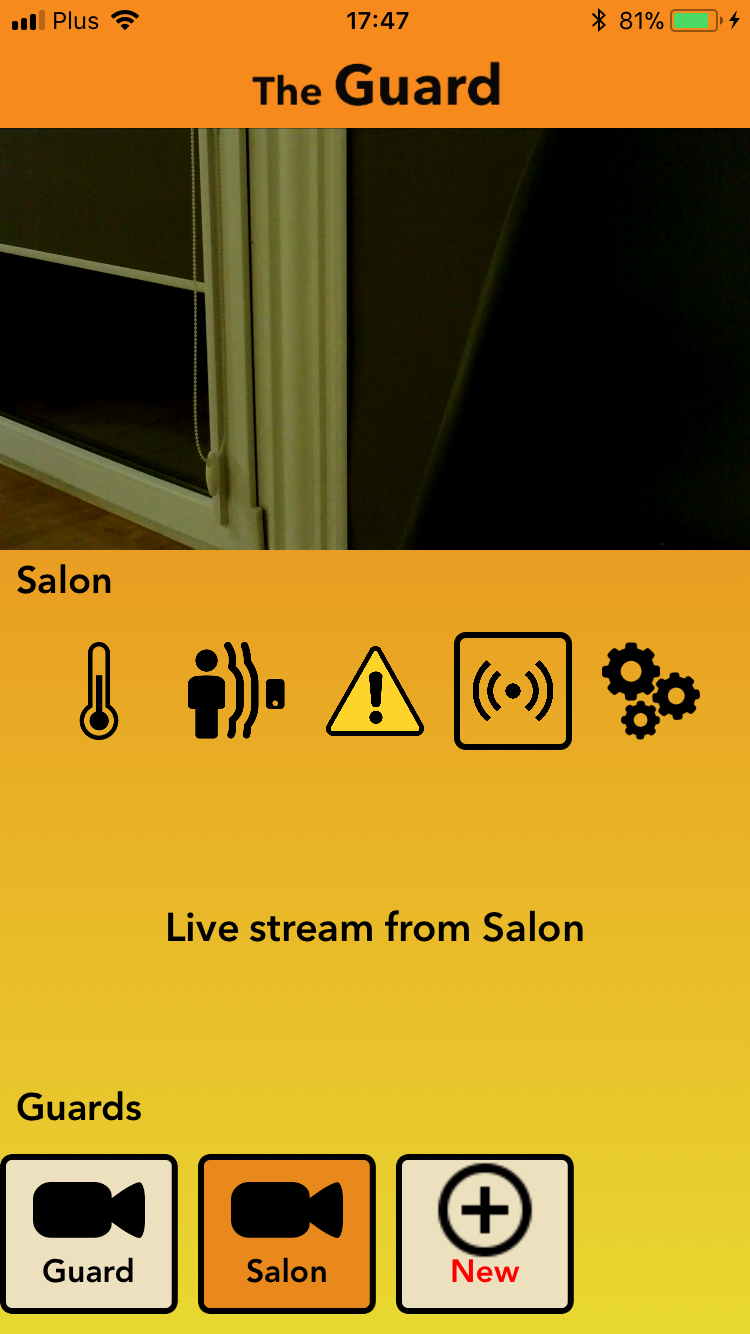
\includegraphics[width=5cm]{ios_screenshots/liveStreamiOS.png}
	\caption{Sekcja monitoringu [źródło własne]}
\end{figure}
\paragraph{Sekcja monitoringu:}
Sekcja odpowiedzialna za prawidłowy odbiór obrazu z kamery zaznaczonej w dolnej części ekranu(rys. 5.x). Okno, w którym odbywa się stream ustawiono w taki sposób, aby bez względu na rozmiar telefonu utrzymywało proporcję 16:9. Pozbyto się dzięki temu czarnych ramek lub braku części transmitowanego obrazu. 
\begin{figure}[ht]
	\centering
	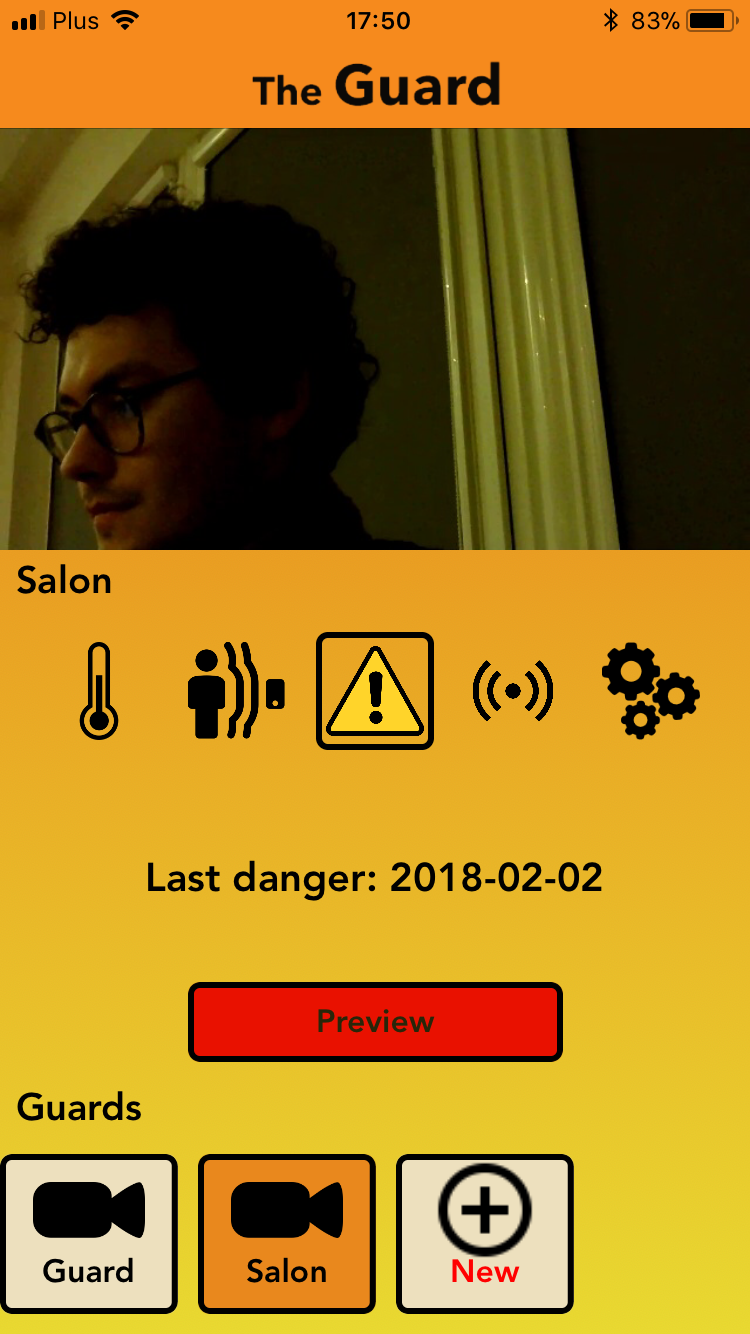
\includegraphics[width=5cm]{ios_screenshots/dangeriOS.png}
	\caption{Sekcja ostatniego zagrożenia [źródło własne]}
\end{figure}

Przeprowadzono kilka testów aplikacji pod pełnym obciążeniem za pomocą programu Instruments. Szczególnie interesująco przedstawia się zużycie sieci podczas streamu obrazu. Widać, że w ciągu jednej minuty pobrano 6,61MB a wysłano jedynie 24,11Kb (rys. 5.8). Obraz pobierany jest tylko wtedy kiedy aplikacja jest aktywna. W ciągu godziny działania aplikacji pobierze ona około 400MB danych. Jednak dla zapewnienia komfortu użytkowania i płynnego streamu obrazu zalecane jest posiadanie łącza umożliwiającego transfer danych na poziomie min. 200KB/s. 
\begin{figure}[ht]
	\centering
	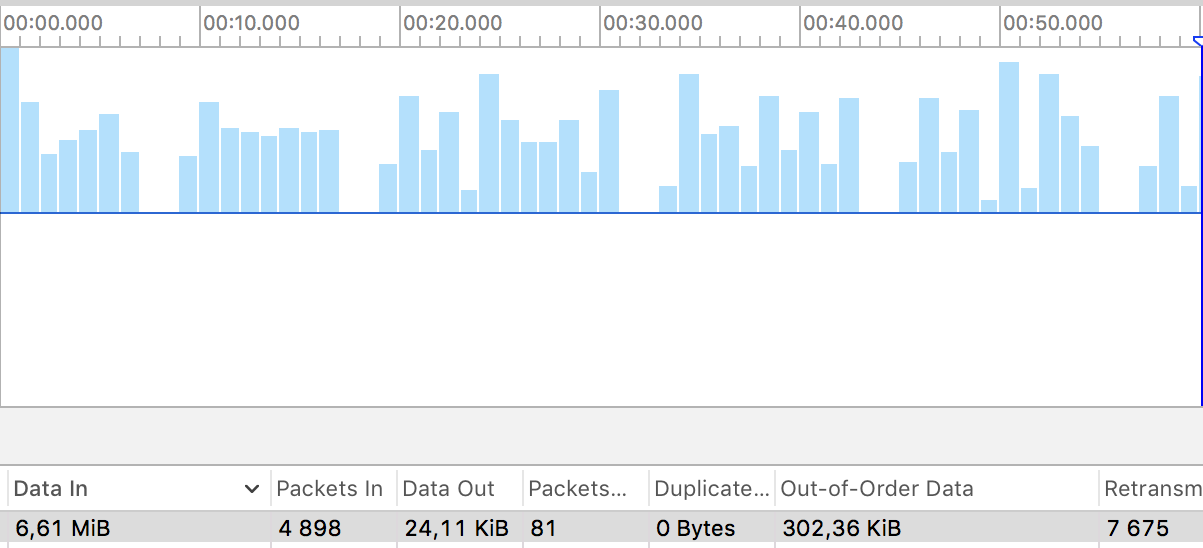
\includegraphics[width=11cm]{ios_screenshots/networkUsage.png}
	\caption{Zużycie sieci podczas streamu [źródło własne]}
\end{figure}
Przeprowadzono także test na zużycie pamięci RAM i zużycie procesora. Te jednak są niewielkie i wynoszą odpowiednio 25MB pamięci RAM i średnio 1 procent zużycia procesora.
Zużycie procesora wzrasta do poziomu ok. 15 procent tylko w momencie pobierania nagranego obrazu z serwera. Wtedy też zużycie pamięci RAM jest o około 5MB większe i wynosi około 30MB (rys. 5.9).
\begin{figure}[ht]
	\centering
	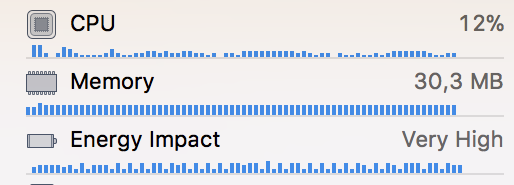
\includegraphics[width=11cm]{ios_screenshots/CPURAM.png}
	\caption{Zużycie procesora i RAM podczas największego obciążenia [źródło własne]}
\end{figure}
Testy przeprowadzono na iPhonie 6S i iPadzie Pro.


\section{Aplikacja internetowa}
Aplikacja webowa przeznaczona jest dla użytkowników wszystkich systemów operacyjnych i~została przetestowana w~przeglądarce Firefox. Rozmieszczenie komponentów aplikacji różni się od tego zastosowanego w~aplikacjach IOS oraz Android - spowodowane jest to inną rozdzielczością ekranu. 

\paragraph{Panel logowania / rejestracji użytkownika:}
\paragraph{Menu wyboru urządzenia:}
\paragraph{Główny panel aplikacji:}
\paragraph{Panel rejestracji urządzenia:}
\paragraph{Panel notyfikacji:}


\paragraph{Implementacja Django - połączenie z bazą danych:}
Biblioteka Django posiada wbudowane rozwiązania umożliwiające pobieranie informacji z bazy danych projektu dzięki czemu aplikacja webowa nie wysyła zapytań na określone dla aplikacji mobilnych porty, tylko komunikuje się bezpośrednio z bazą danych. Rozwiązanie to umożliwia uniezależnienie aplikacji webowej od stanu portów oraz zmniejsza liczbę potrzebnych zapytań wysyłanych do serwera.
Aplikacja internetowa przeznaczona jest dla użytkowników wszystkich systemów operacyjnych i~została przetestowana w~przeglądarce Firefox w systemach operacyjnych Microsoft Windows 10 oraz Linux Debian 9 (Firefox ESR 52.5.2 64 bit). Do stworzenia aplikacji użyto języków programowania Python 3, JavaScript oraz framework'u Django, natomiast frontend jest oparty na bibliotece Bootstrap oraz JQuery. Połączenie z~bazą danych Firebase zaimplementowano za pomocą Firebase Web Api. Rozmieszczenie komponentów aplikacji różni się od tego zastosowanego w~aplikacjach IOS oraz Android - spowodowane jest to inną rozdzielczością ekranu. 

\paragraph{Panel logowania / rejestracji użytkownika:} Panele logowania oraz rejestracji użytkownika są do siebie bardzo podobne - jedyna ich różnica jest w nazwie i~funkcjonalności. Obydwa panele składają się z~loga aplikacji oraz formularza w~którym trzeba podać adres email i~hasło. W przypadku panelu logowania, dane są weryfikowane i~jeśli są poprawne użytkownik zostaje zalogowany. Jeżeli użytkownik chce zarejestrować konto, sprawdzana jest poprawność adresu email, a następnie tworzone jest konto w usłudze FireBase Auth. W przypadku błędu, jest on wyświetlany powyżej formularza (rys. \ref{web_login})

\paragraph{Menu wyboru urządzenia:} Po prawidłowym zalogowaniu do aplikacji, użytkownik może zobaczyć listę swoich urządzeń, dodać nowe oraz zaczyna dostawać powiadomienia w razie wykrytego zagrożenia. W~przypadku kliknięcia przycisku `Connect rasp', użykownik zostaje przekierowany do widoku umożliwiającego rejestrację nowego urządzenia(rys. \ref{web_register}). Po wprowadzeniu numeru seryjnego urządzenia oraz jego nazwy, zostaje dodany do baz danych. Po wybraniu urządzenia, informacje nt. jego stanu będą wyświetlane po prawej stronie okna, która w momencie zalogowania jest pusta (rys. \ref{web_main_page}). Urządzenia w~menu są rozpoznawane na podstawie ich nazw. 

\paragraph{Widok konkretnego urządzenia:} Po wybraniu z~menu kokretnego urządzenia, użytkownik zostaje przekierowany na stronę pojedyńczego urządzenia (rys. \ref{web_rasp_view}). Pod nazwą urządzenia i~jego numerem seryjnym wyświetlany jest aktualny obraz z kamery oraz stan czujników. Dzięki zastosowaniu nasłuchiwania na bazie danych Firebase, zmiany są na bieżąco wyświetlane na stronie. Użytkownik ma możliwość po naciśnięciu odpowiedniego przycisku:
\begin{itemize}
\item Zmienić nazwę urządzenia - po kliknięciu na przycisk rename znajdujący się obok nazwy urządzenia, użytkownik zostanie przekierowany do panelu zmiany nazwy (rys. \ref{web_rasp_rename}).
\item Wyłączyć / włączyć alerty 
\item Zobaczyć notyfikacje danego urządzenia - poprzez klknięcie na przycisk `Check notifications from this device', użytkownik zostanie przekierowany do widoku listy notyfikacji danego urządzenia (rys. \ref{web_rasp_notifications}).
\end{itemize}

\paragraph{Wyświetlanie notyfikacji:} W każdym z widoków aplikacji webowej w czasie rzeczywistym sprawdzane są notyfikacje z bazy danych z pomocą Firebase WebApi. W przypadku wykrycia zmiany uznawanej za niebezpieczną za pomocą skryptów przeglądarki (JavaScript + JQuery) wyświetlany jest monit informujący o niebezpiecznym zdarzeniu, co pokazane jest na rysunku \ref{web_rasp_notifications}.  

\paragraph{Implementacja Django - połączenie z bazą danych:}
Biblioteka Django posiada wbudowane rozwiązania umożliwiające pobieranie informacji z bazy danych projektu dzięki czemu aplikacja webowa nie wysyła zapytań na określone dla aplikacji mobilnych porty, tylko komunikuje się bezpośrednio z bazą danych. Rozwiązanie to umożliwia uniezależnienie aplikacji webowej od stanu portów oraz zmniejsza liczbę potrzebnych zapytań wysyłanych do serwera.
Aplikacja internetowa przeznaczona jest dla użytkowników wszystkich systemów operacyjnych i~została przetestowana w~przeglądarce Firefox w systemach operacyjnych Microsoft Windows 10 oraz Linux Debian 9 (Firefox ESR 52.5.2 64 bit). Do stworzenia aplikacji użyto języków programowania Python 3, JavaScript oraz framework'u Django, natomiast frontend jest oparty na bibliotece Bootstrap oraz JQuery. Połączenie z~bazą danych Firebase zaimplementowano za pomocą Firebase Web Api. Rozmieszczenie komponentów aplikacji różni się od tego zastosowanego w~aplikacjach IOS oraz Android - spowodowane jest to inną rozdzielczością ekranu. 

\paragraph{Panel logowania / rejestracji użytkownika:} Panele logowania oraz rejestracji użytkownika są do siebie bardzo podobne - jedyna ich różnica jest w nazwie i~funkcjonalności. Obydwa panele składają się z~loga aplikacji oraz formularza w~którym trzeba podać adres email i~hasło. W przypadku panelu logowania, dane są weryfikowane i~jeśli są poprawne użytkownik zostaje zalogowany. Jeżeli użytkownik chce zarejestrować konto, sprawdzana jest poprawność adresu email, a następnie tworzone jest konto w usłudze FireBase Auth. W przypadku błędu, jest on wyświetlany powyżej formularza (rys. \ref{web_login})

\paragraph{Menu wyboru urządzenia:} Po prawidłowym zalogowaniu do aplikacji, użytkownik może zobaczyć listę swoich urządzeń, dodać nowe oraz zaczyna dostawać powiadomienia w razie wykrytego zagrożenia. W~przypadku kliknięcia przycisku `Connect rasp', użykownik zostaje przekierowany do widoku umożliwiającego rejestrację nowego urządzenia(rys. \ref{web_register}). Po wprowadzeniu numeru seryjnego urządzenia oraz jego nazwy, zostaje dodany do baz danych. Po wybraniu urządzenia, informacje nt. jego stanu będą wyświetlane po prawej stronie okna, która w momencie zalogowania jest pusta (rys. \ref{web_main_page}). Urządzenia w~menu są rozpoznawane na podstawie ich nazw. 

\paragraph{Widok konkretnego urządzenia:} Po wybraniu z~menu kokretnego urządzenia, użytkownik zostaje przekierowany na stronę pojedyńczego urządzenia (rys. \ref{web_rasp_view}). Pod nazwą urządzenia i~jego numerem seryjnym wyświetlany jest aktualny obraz z kamery oraz stan czujników. Dzięki zastosowaniu nasłuchiwania na bazie danych Firebase, zmiany są na bieżąco wyświetlane na stronie. Użytkownik ma możliwość po naciśnięciu odpowiedniego przycisku:
\begin{itemize}
\item Zmienić nazwę urządzenia - po kliknięciu na przycisk rename znajdujący się obok nazwy urządzenia, użytkownik zostanie przekierowany do panelu zmiany nazwy (rys. \ref{web_rasp_rename}).
\item Wyłączyć / włączyć alerty 
\item Zobaczyć notyfikacje danego urządzenia - poprzez klknięcie na przycisk `Check notifications from this device', użytkownik zostanie przekierowany do widoku listy notyfikacji danego urządzenia (rys. \ref{web_rasp_notifications}).
\end{itemize}

\paragraph{Wyświetlanie notyfikacji:} W każdym z widoków aplikacji webowej w czasie rzeczywistym sprawdzane są notyfikacje z bazy danych z pomocą Firebase WebApi. W przypadku wykrycia zmiany uznawanej za niebezpieczną za pomocą skryptów przeglądarki (JavaScript + JQuery) wyświetlany jest monit informujący o niebezpiecznym zdarzeniu, co pokazane jest na rysunku \ref{web_rasp_notifications}.  

\paragraph{Implementacja Django - połączenie z bazą danych:}
Biblioteka Django posiada wbudowane rozwiązania umożliwiające pobieranie informacji z bazy danych projektu dzięki czemu aplikacja webowa nie wysyła zapytań na określone dla aplikacji mobilnych porty, tylko komunikuje się bezpośrednio z bazą danych. Rozwiązanie to umożliwia uniezależnienie aplikacji webowej od stanu portów oraz zmniejsza liczbę potrzebnych zapytań wysyłanych do serwera.

    \chapter{Testy funkcjonalne}

Testy:
 * Rejestracja+dodanie raspa
 * Aplikacji (3x, dla każdej):
 ** Sprawdzenie zagrożenia (skok wartości jednego z czujników)
 ** Sprawdzenie obrazu z kamery na wybranym raspie
 ** Odtworzenie nagrania video

\chapter{Uwagi końcowe}

Grupa zrealizowała wszystkie cele postawione sobie na początku pracy. Wykonany system działa i jest przystosowany do dalszej modyfikacji. Istnieje możliwość wymiany czujników z rodziny MQ na inne bez konieczności zmian w oprogramowaniu uruchomionym na Raspberry, ze względu na podobny charakter ich działania. W następnej fazie zalecane byłoby zaprojektowanie lepszej obudowy na czujniki aby poprawić design systemu. Zdecydowano, że cały system będzie na licencji open-source, aby każdy mógł pobrać oprogramowanie i edytować je według własnych potrzeb. Mimo, że taktowanie procesora Raspberry Pi 3 nie jest wysokie i nie poradziłby on sobie sam z zadaniami przedstawionymi na początku pracy to dzięki zastosowaniu zewnętrzych serwerów i usług na takich platformach jak Microstof Azure udało się wykonać w pełni działający system bezpieczeństwa. Przeniesiono bardzo obciążające zadania takie jak przetwarzanie obrazu na zewnętrzne platformy, które wyposażone są w znacznie bardziej zaawansowane podzespoły. Wykorzystanie natomiast usług Firebase, z którego korzystają też takie firmy jak Trivago czy Shazam pozwoliło na szybką implementację zaawansowanych funkcji takich jak uwierzytelnianie użytkowników czy aktualizację zmian w bazie danych w czasie rzeczywistym. Grupa zamierza dalej pracować nad systemem kontroli bezpieczeństwa - The Guard aby uczynić świat lepszym a przede wszystkim bezpieczniejszym miejscem do życia :)


// TODO Remove dummy doc links
\cite{MDESIGN}
\cite{RXJAVA}
\cite{KOTLIN}
\cite{RPI}
\cite{firebase}
\cite{android}
\cite{azure}
\cite{kotlin}

    
  %  {\raggedright\sloppy\small\bibliography{bibliography}}
    \cleardoublepage
    \begingroup
    \makeatletter
    \let\ps@plain\ps@plain
    \makeatother
    
    \pagestyle{plain}

    % Bibliography (books, articles) starts here.
    \bibliographystyle{unsrt} 
    \bibliography{bibliography}     
    \listoffigures
    \pagestyle{plain}
    \cleardoublepage
    \endgroup
    
    % Colophon is a place where you should let others know about copyrights etc.
    \ppcolophon

\end{document}
